\documentclass[11pt,a4paper]{ivoa}
\input tthdefs
\input gitmeta

\usepackage{graphicx}
\usepackage{longtable}
\usepackage{booktabs}
\usepackage{amsmath}
\usepackage{hyperref}
\usepackage{enumitem}
\usepackage{todonotes}
\usepackage{tcolorbox}

\title{HiPS -- Hierarchical Progressive Survey}
\ivoagroup{Applications}

\author{{\em ToBeCompletedAndConfirmed:}}
\author{Pierre Fernique (CDS)}
\author{Mark Allen(CDS)}
\author{Deborah Baines (ESA)}
\author{Matthieu Baumann (CDS)}
\author{Thomas Boch (CDS)}
\author{Caroline Bot (CDS)}
\author{Tom Donaldson (STScI/NASA)}
\author{Daniel Durand (CADC)}
\author{Ken Ebisawa (JAXA)}
\author{Laurent Michel (Observatoire Astronomiques de Strasbourg)}
\author{Henrik Norman (Winter Way for ESA)}
\author{François-Xavier Pineau (CDS)}
\author{Thomas Robitaille}
\author{Jesus Salgado (SKAO)}
\author{Felix Stoehr (ALMA/ESO)}

\editor{Pierre Fernique}
%\date{2025-11-15}

\previousversion[https://www.ivoa.net/documents/HiPS/20170519]{Version1.0}

\begin{document}
\begin{abstract}
This document presents HiPS, a hierarchical scheme for the description, storage and access of sky survey data. The system is based on hierarchical tiling of sky regions at finer and finer spatial resolution which facilitates a progressive view of a survey, and supports multi-resolution zooming and panning. HiPS is based on a HEALPix discretization of the sphere. This second edition of the document extends this discretization principle to a potential second physical dimension: time or frequency. HiPS is implemented as a simple file structure with a direct indexing scheme, which allows for practical implementations. It is implemented as a simple file structure with a direct indexing scheme that leads to practical implementations.
\end{abstract}

\listoffigures
\listoftables  

\section*{Acknowledgments}
We acknowledge support from the Astronomy ESFRI and Research Infrastructure Cluster – ASTERICS project, funded by the European Commission under the Horizon 2020 Programme (GA 653477) - the SKA SRCNet project as part of collaborative developments for the Square Kilometre Array Observatory (SKAO).

\section*{Conformance-related definitions}

The words ``MUST'', ``SHALL'', ``SHOULD'', ``MAY'', ``RECOMMENDED'', and
``OPTIONAL'' (in upper or lower case) used in this document are to be
interpreted as described in IETF standard RFC2119 \citep{std:RFC2119}.

The \emph{Virtual Observatory (VO)} is a
general term for a collection of federated resources that can be used
to conduct astronomical research, education, and outreach.
The \href{https://www.ivoa.net}{International
Virtual Observatory Alliance (IVOA)} is a global
collaboration of separately funded projects to develop standards and
infrastructure that enable VO applications.

\section{Introduction}

This document describes the Hierarchical Progressive Survey (HiPS) system for access and visualization of astronomical survey data. The aim of the HiPS system is to enable dedicated client/browser tools to access and display an astronomical survey progressively, based on the principle that {\em "the more you zoom in on a particular area the more details show up"}.

\begin{figure}[h]
\begin{center}
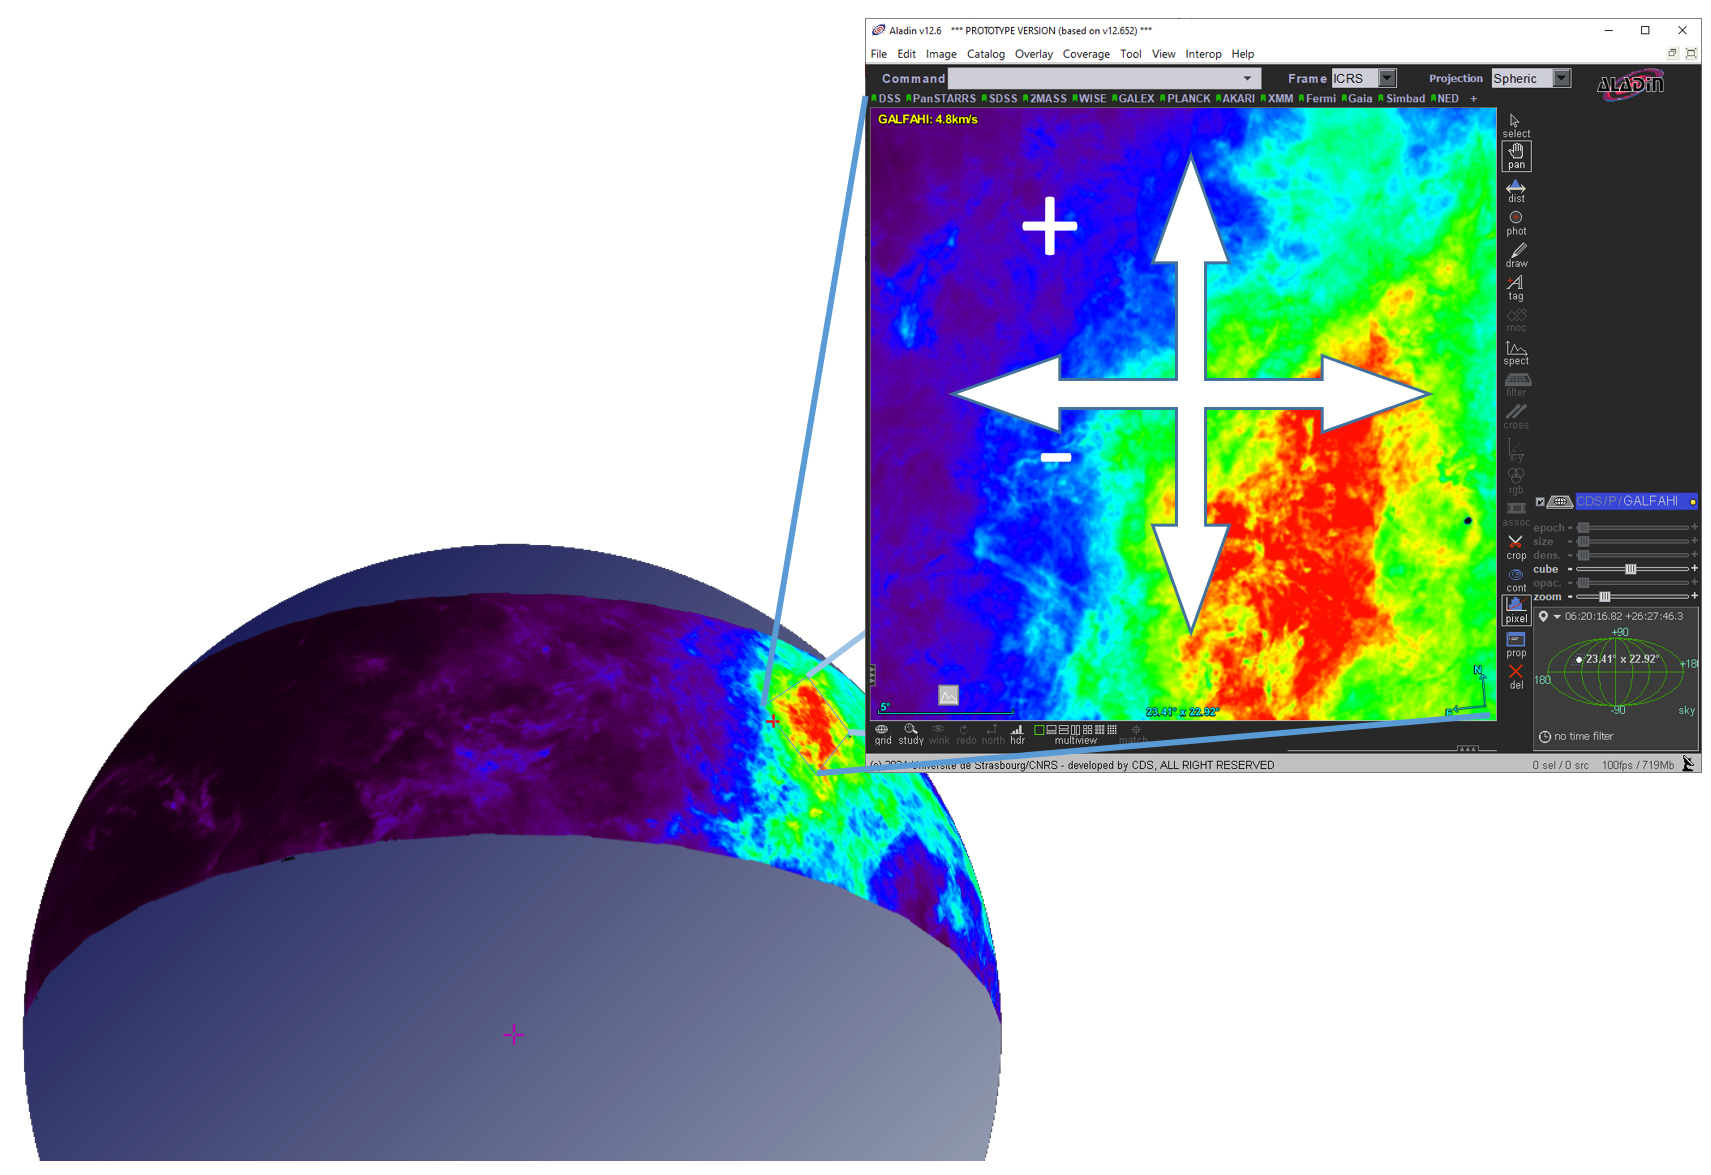
\includegraphics[width=\textwidth]{HiPS-f1.png}
\end{center}
\caption{HiPS spherical  browsing principle }
\label{fig:fig1}
\end{figure}

\begin{figure}[h]
\begin{center}
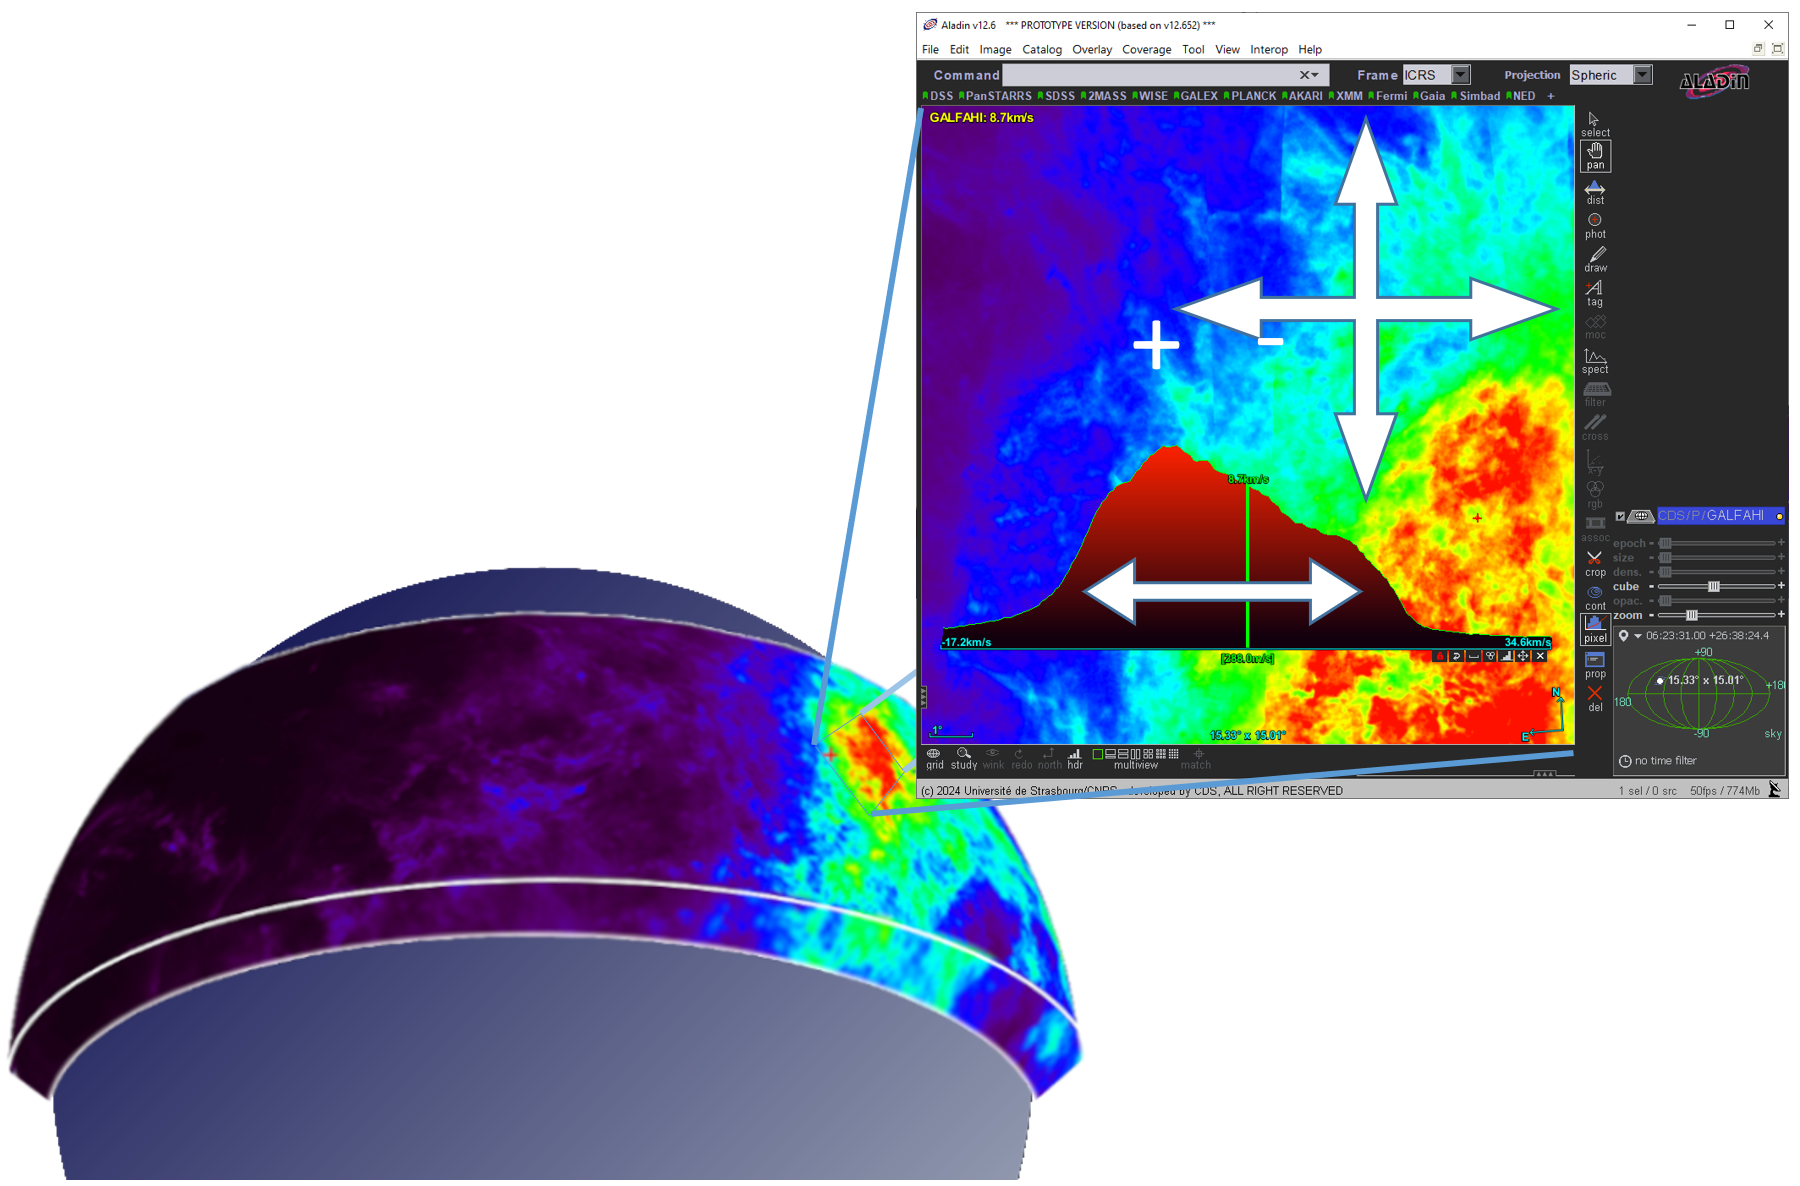
\includegraphics[width=\textwidth]{HiPS-f1a.png}
\end{center}
\caption{HiPS spherico-cubic browsing principle }
\label{fig:fig1}
\end{figure}


We adopt the term ‘astronomical survey’ in a broad sense to include: all-sky surveys, cubic surveys, collections of pointed observations, catalogues of sources. In principle HiPS can manage any types of data that can be located and displayed on the sphere. Thus, we will use the general terms “spherical surveys” or “spherical-cubic survey.”. HiPS is designed specifically for astronomical data in that it takes the physical properties (astrometric, frequency, time, photometric, etc) of the original data into account, and emphasis is placed on ease of use without the need for special servers or database systems.

The full context and motivation of HiPS is described in \cite{Fernique2015}. HiPS was originally designed by CDS (Centre de Données astronomiques de Strasbourg) in 2010 in the framework of the Aladin project whereupon its popularity has rapidly overtaken the original scope. The emergence of several independent HiPS clients and servers has been the main motivation to standardize this method in the IVOA framework as a first version of this document - HiPS1.0 (2017) - focused on spatial spherical data.  This second version - HiPS2.0 - enhances the original approach to enable hierarchical approach for large spherical-cubic surveys such as SKA survey \citep{SKA2024}. These additions and extensions remain fully compatible with the recommendations in version 1 (see appendix~\ref{sec:history} for details of the enhancements). 

Essentially, HiPS describes a generic method for packaging, storing, querying, and describing astronomical data. In other terms, HiPS is designed for celestial observations but can also be used for planetary surfaces observations, or any other data described in a spherical or cubico-spherical coordinates. 

There are dependencies on other VO standards, notably MOC \citep{MOC2.1}, the VOResource  \citep{2008ivoa.spec.0222P}, the IVOA Identifier \citep{2016ivoa.spec.0523D}, the ObsCoreDM \citep{2017ivoa.spec.0509L} and VOTable \citep{2019ivoa.spec.1021O}. HIPS is also based on other non-IVOA standards notably HEALPix \citep{Gorski2005} and FITS \citep{FITS}, as well as the JPEG and PNG image formats.



\subsection{Role within the VO Architecture}

\begin{figure}
\centering

% As of ivoatex 1.2, the architecture diagram is generated by ivoatex in
% SVG; copy ivoatex/archdiag-full.xml to role_diagram.xml and throw out
% all lines not relevant to your standard.
% Notes don't generally need this.  If you don't copy role_diagram.xml,
% you must remove role_diagram.pdf from SOURCES in the Makefile.

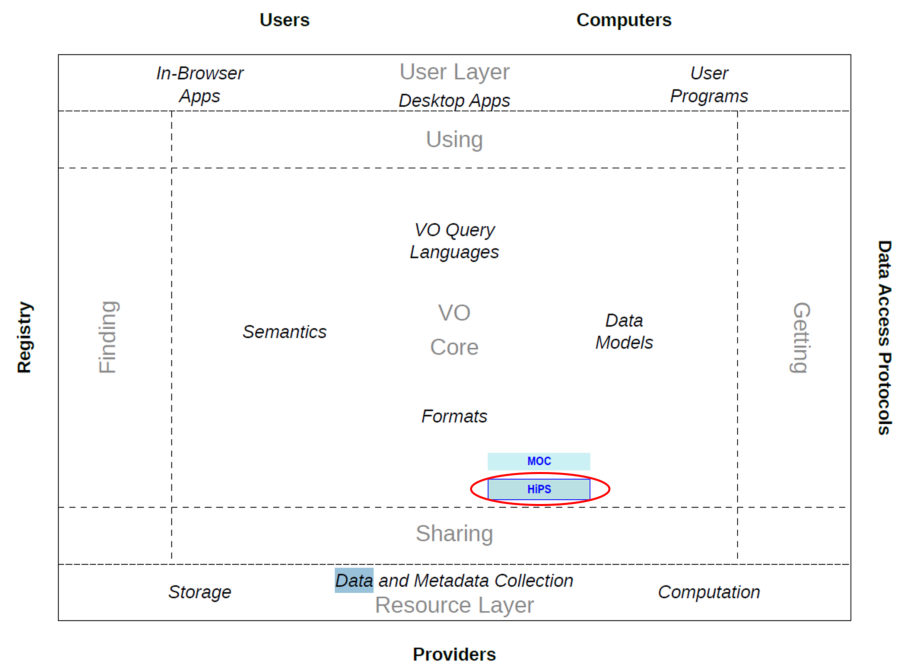
\includegraphics[width=0.9\textwidth]{role_diagram.pdf}
\caption{Architecture diagram for this document}
\label{fig:archdiag}
\end{figure}

Fig.~\ref{fig:archdiag} shows the role this document plays within the
IVOA architecture \citep{2021ivoa.spec.1101D}.


\section{Usage examples}

The most common usage of HiPS is the visualisation of data from large astronomical surveys. HiPS allows one to browse "big data": pan and zoom into each section of the survey data using HiPS clients that access the data over the internet. Only the portion of the data needed for the current user view is streamed from the server to the client. This remote visualisation technique enables the exploration of large data sets from a wide field of view where an entire survey is projected on the whole sky, to a detailed zoomed view at the finest spatial resolution of the images used for the survey.

\begin{figure}[h]
\begin{center}
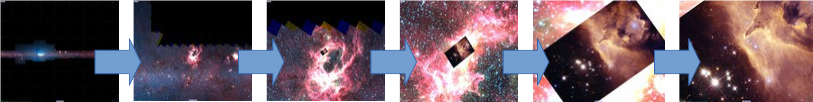
\includegraphics[width=\textwidth]{HiPS-f2.png}
\end{center}
%\caption{ }
\label{fig:fig2}
\end{figure}

This visualisation technique is not limited to pixel surveys but may also be used for other data types: source catalogues, pixel cubes, etc. For example, the HiPS scheme can be used to describe a multiresolution view of a source catalogue where the selection of catalogue points is a representation of different parameters like brightness. This allows a different view of the catalogue at different zoom level. For example we could display fainter and fainter sources as one zooms into higher orders of the map. As such, HiPS catalogues can provide a hierarchical view of catalogues where the hierarchy can be based on a selected quantitative property for each catalogue.

\begin{figure}[h]
\begin{center}
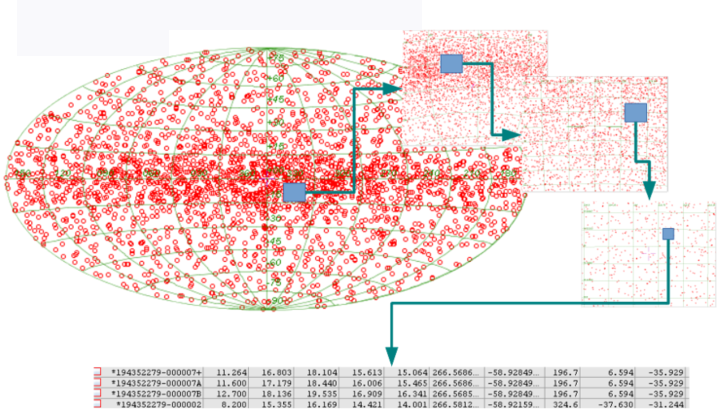
\includegraphics[width=\textwidth]{HiPS-f3.png}
\end{center}
\caption{HiPS catalog visualisation example (GAIA-GUMS catalog)}
\label{fig:fig3}
\end{figure}

The HiPS scheme can also be used for multiresolution visualization of cubic data, especially spatio-temporal or spatio-frequencial data, allowing the principle of zooming and panning to be applied to all physical dimensions simultaneously.

\begin{figure}[h]
\begin{center}
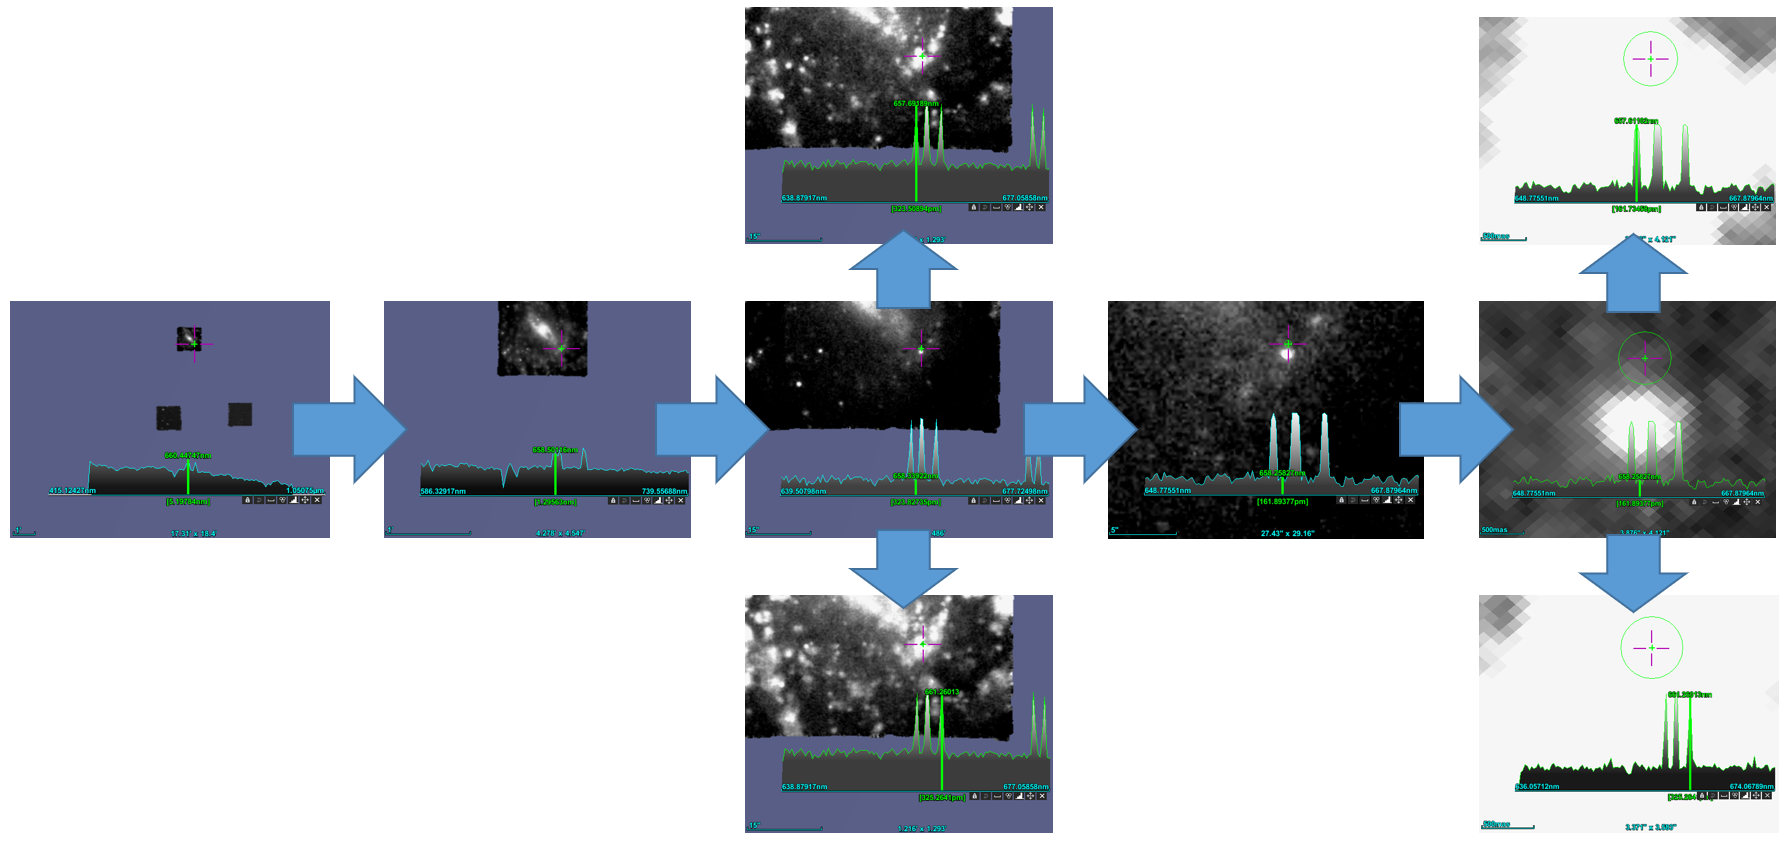
\includegraphics[width=\textwidth]{HiPS-f4.png}
\end{center}
\caption{HiPS cube visualisation example (MUSE survey)}
\label{fig:fig4}
\end{figure}

\section{HiPS principle}

HiPS uses the Hierarchical Equal Area isoLatitude Pixelization tessellation technique (HEALPix) for applying a sperical spatial discretization. The motivations for using  the HEALPix tessellation have already been discussed in the MOC IVOA standard  document in section 1.4 \citep{MOC2016}. The main arguments in favour of HEALPix are the equal area property, the fast and constant computation time which does not depend on the hierarchical level, the accuracy and performance of the available libraries (0.4 mas), and the wide usage of HEALPix in several sky missions (WMAP, PLANCK, LIGO…).

HEALPix is a curvilinear partitioning of the sphere that supports a hierarchical tree structure for multi-resolution applications. The detailed geometry and properties of HEALPix are described in \cite{Gorski2005}. The HEALPix partitioning of the sphere has a base resolution that divides the sphere into 12 cells, each of which is sub-divided into 4 cells recursively. Thus the sphere at order 1 consists of 48 cells, 192 cells at order 2, 768 at order 3 and so on.  Each cell at a given level covers an equal area of the sphere.

\begin{figure}[h]
\begin{center}
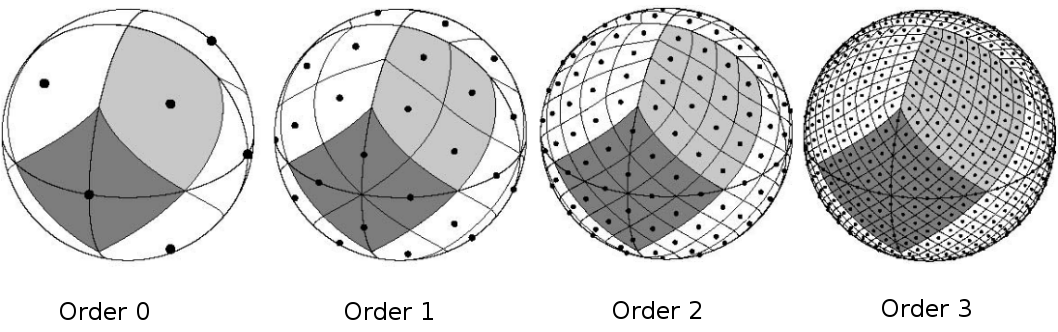
\includegraphics[width=\textwidth]{HiPS-f5.png}
\end{center}
\caption{Spatial HiPS partitioning based on HEALPix}
\label{fig:fig5}
\end{figure}

HiPS is essentially a mapping of survey data at various spatial resolutions into a collection of HiPS tiles stored in regular files inside a basic file system. 

The HiPS tiles define the basic unit of storage. They contain the data (pixels for images, astronomical objects for catalog, etc) spatially organized in the corresponding HEALPix cell. Each HiPS tile is fully identified and localized on the sphere by its address composed by its HEALPix order and its HEALPix cell index.

The HiPS principle is extended to cubic data by mapping them both spatially based on HEALPix tessellation and on the additional physical axis (time, frequency, ...). HiPS tiles will therefore have a thickness and will be identified by the address composed by the HEALPix cell order and index on the one hand, and by the order and index of the cell resulting from the discretization of the additional physical axis on the other hand.

\begin{figure}[h]
\begin{center}
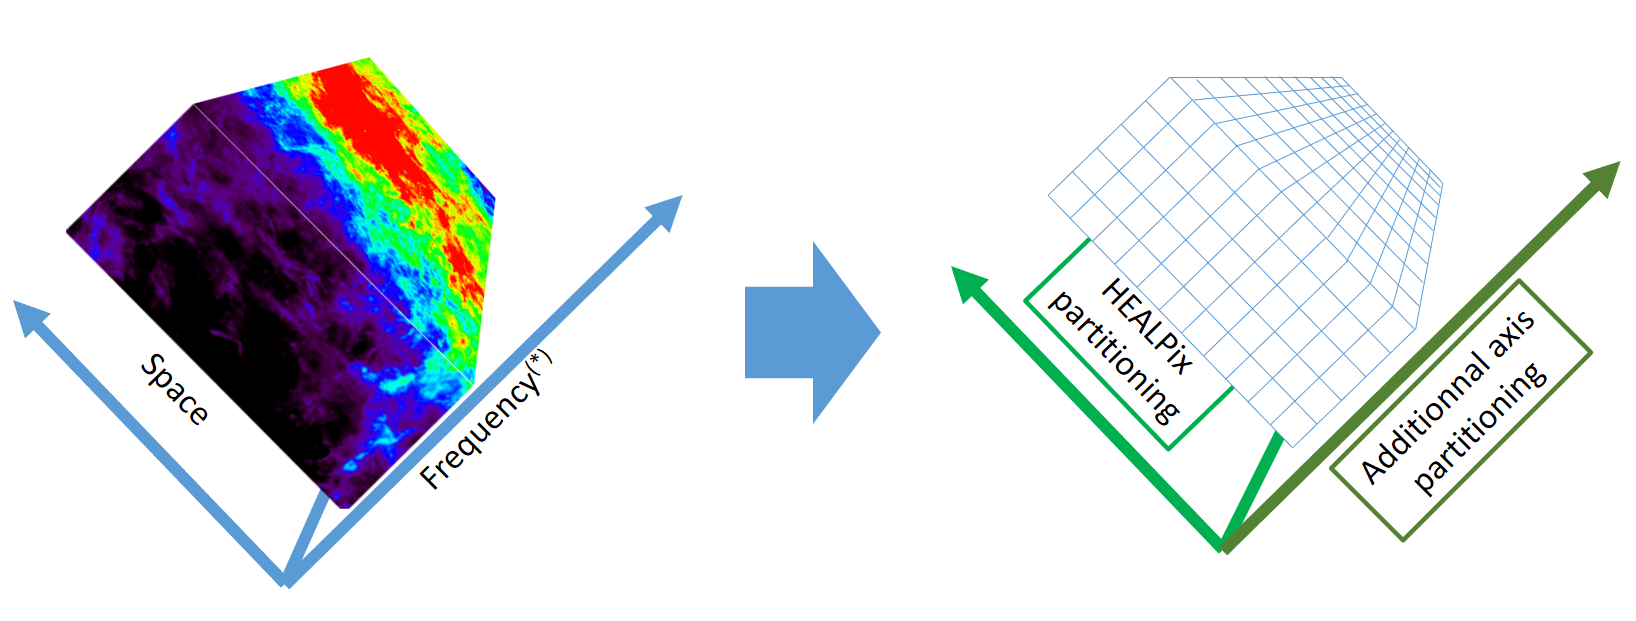
\includegraphics[width=\textwidth]{HiPS-f6.png}
\end{center}
\caption{HiPS cube partitioning pinciple}
\label{fig:fig6}
\end{figure}

\medskip


The next two sections of this document are normative. Respectively, they present the HiPS encoding method (section~\ref{sec:encoding}), the HiPS distribution and registration protocol (section~\ref{sec:distribution}), and the HiPS client access and use procedures (section~\ref{sec:use}). 

\medskip

To facilitate understanding of this document, we introduce below the HiPS-specific vocabulary:

\begin{tcolorbox}

\begin{itemize}[noitemsep,topsep=0pt,parsep=0pt,partopsep=0pt]
\item {\bf HiPS}: Hierarchical Progressive Survey:\\
    - {\bf HiPS image}: HiPS method applied for image collection\\
    - {\bf HiPS catalog}: HiPS method applied for catalogues\\
    - {\bf HiPS cube}: Generalization of the HiPS method to cubic data, also known as {\bf HiPS3D} prior to its IVOA standardization.
\item {\bf cell:} HiPS partitioning element (synonym of {\em pixels}):\\
    - Spatial case: HEALPix diamond (constant surface for a given order)\\
    - Temporal case: time interval (constant duration for a given order)\\
    - Frequency case: frequency interval (logarithmic interval for a given order)
\item {\bf pixel:} synonym of {\em cell}.
\item {\bf tile}: group of "adjacent" HiPS {\em pixels} (according to HiPS rule)\\
    - {\bf width}: number of linearly grouped {\em pixels} (in time and frequency), and number of {\em pixels} on one side (in space)\\
    - {\bf depth}: number of tile channels in HiPS cube\\
\item {\bf address}: Composite number used to identify and localize a HiPS {\em cell} or {\em tile}. It is composed of 2 values: {\em order} and {\em index}.\\
    - {\bf order}: HiPS order\\
    - {\bf index}: the pixel number in the specified {\em order}  (synonym of {\em npix})\\
   In the case of HiPS cube, 2 additional values are added to the {\em address}:\\
    - {\bf orderZ}: frequency (respectively time) {\em order}\\
    - {\bf indexZ}: the pixel's frequency (or time) number in the specified {\em orderZ}\\
    A such {\em address} may be written as follows:\\
   {\tt order/index} and {\tt order/index\_orderZ/indexZ} for HiPS cube.
\item {\bf npix}: synomym of {\em index}
\item {\bf HiPS node}: HTTP server in charge of providing one or more HiPS 
\item {\bf HiPS server}: synonym of {\em HiPS node}
\item {\bf HiPS list}: Standardized list of HiPS provided by a {\em HiPS node}
\item {\bf HiPS client}: Software dedicated to display and/or operate HiPS
\end{itemize}

\end{tcolorbox}


\section{HiPS encoding}
\label{sec:encoding}

This section describes the structure of HiPS data: the format and the architecture of the HiPS tiles. This takes into account the nature of surveys (images, catalogues, cubes, etc) - and the associated metadata elements provided with HiPS.

HiPS generated from spatial data (images, catalogs) are described in the first subsection. The extension to cubic data is then described.

\subsection{Spatial data}
\label{sec:spatial}

Spatial data encoding involves mapping all observation elements (pixels or catalogue sources) onto a HEALPix grid, enabling them to be grouped and manipulated hierarchically as directly addressable tiles.

\begin{figure}[h]
\begin{center}
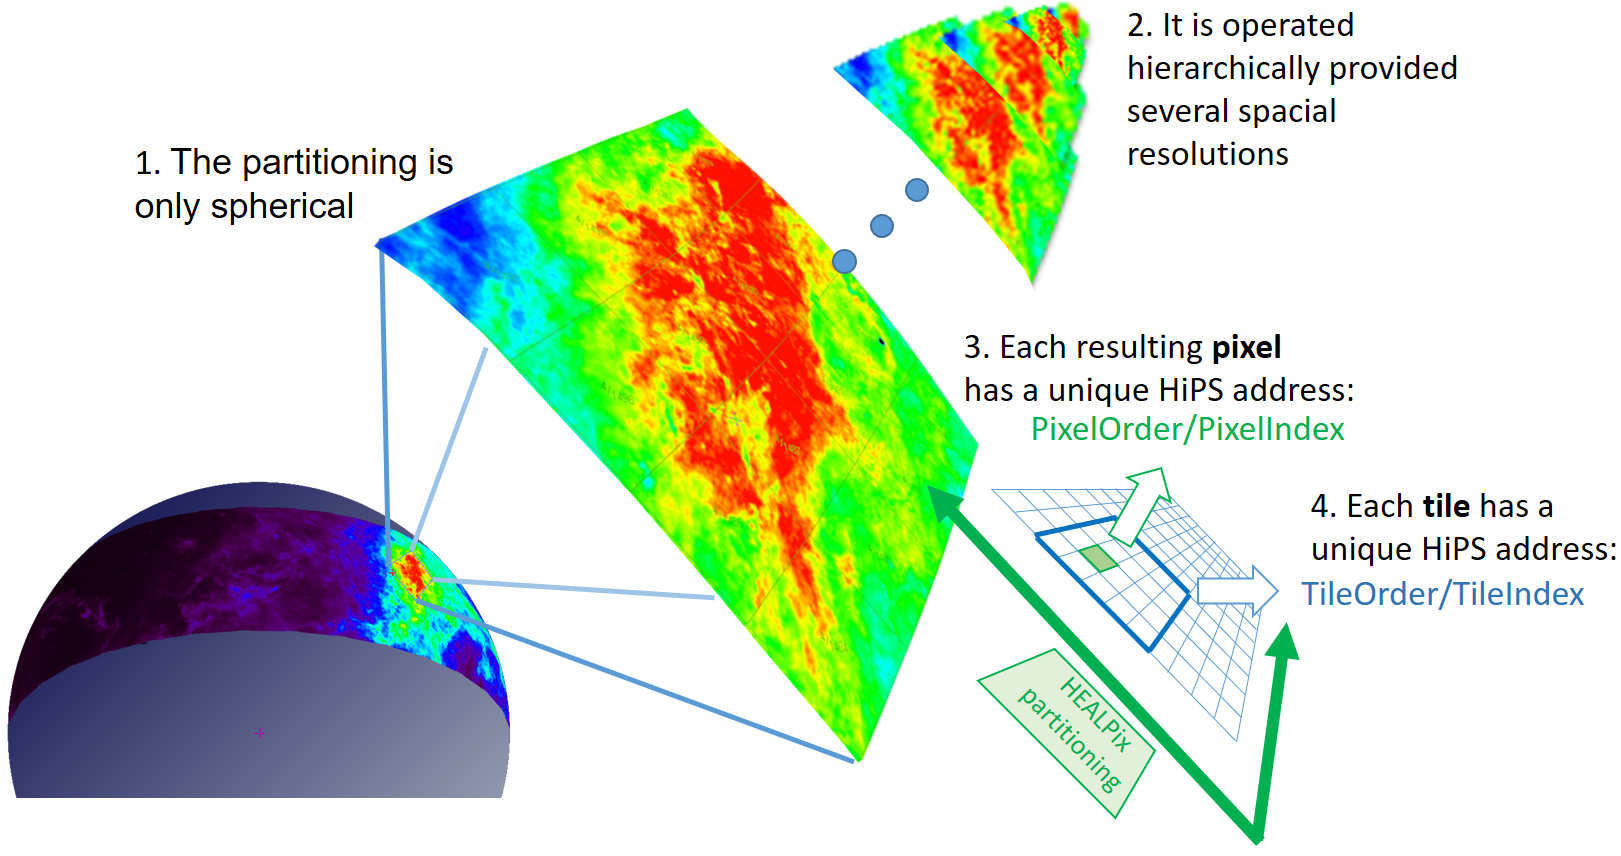
\includegraphics[width=\textwidth]{HiPS-f6a.png}
\end{center}
\caption{HiPS spherical discretization principle }
\label{fig:fig1}
\end{figure}

\subsubsection{Directory structure}
\label{sec:directory}

The tiles used by a HiPS for packaging spatial pixel resulting from the discretization must be visible as a collection of files in a directory tree. The structure of these directories must follow the hierarchy: order $\rightarrow$ tiles, by using respectively the prefix "Norder" for tile orders, and "Npix" for tile indices. To avoid directories becoming too large, the tiles must be grouped by 10,000 items, using the subdirectory prefix "Dir". 

Formally, the tile of address {\tt K/N} - i.e. index N in order K - is located in the HiPS directory structure by this rule:

\medskip
\noindent\fbox{%
\parbox{0.98\linewidth}{%
\begin{center}
Tile K/N $\rightarrow$ \texttt{NorderK/DirD/NpixN\{.ext\}}
\end{center}
where $D = \lfloor N//10000 \rfloor \times 10000$ (//:integer division), \\
and \texttt{\{.ext\}} depends on the nature of the survey (see ``tile format'' below).
}}
\medskip

\medskip
\noindent\textit{Example: the tile containing the HiPS data corresponding to the HEALPix cell index 10302 at the order 6 will be stored in the file\\Norder6/Dir10000/Npix10302{.ext}}
\medskip

\begin{figure}[h]
\begin{center}
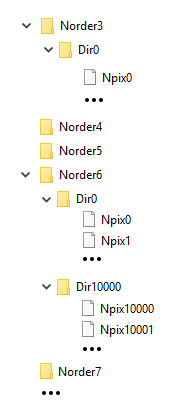
\includegraphics[width=0.3\textwidth]{HiPS-f7.png}
\end{center}
\caption{Example of HiPS directory and file structure}
\label{fig:fig7}
\end{figure}

The spatial location on the sphere of any tile (center of the tile, corners, etc) is directly computed from the tile index using HEALPix formulae \citep{Gorski2005}. 

Following the HEALPix geometry, there are four times more tiles at order $K+1$ compared to the order K. Even if HEALPix supports both "NESTED" and "RING" numbering schemes. HiPS must use the NESTED numbering scheme only. Thus, the tile index N at order K corresponds to the 4 tile indices $N \times 4$, $N \times 4+1$, $N \times 4+2$ and $N \times 4+3$ at order $K+1$.

The actual implementation of HiPS as directories and files is not an obligation, only the view as directories and files is required (see HiPS distribution section). Internally, a HiPS may be stored in a data base, or any other appropriate packaging (tar, zip or dedicated binary files…) rather than in a basic file system directory structure.

\begin{figure}[h]
\begin{center}
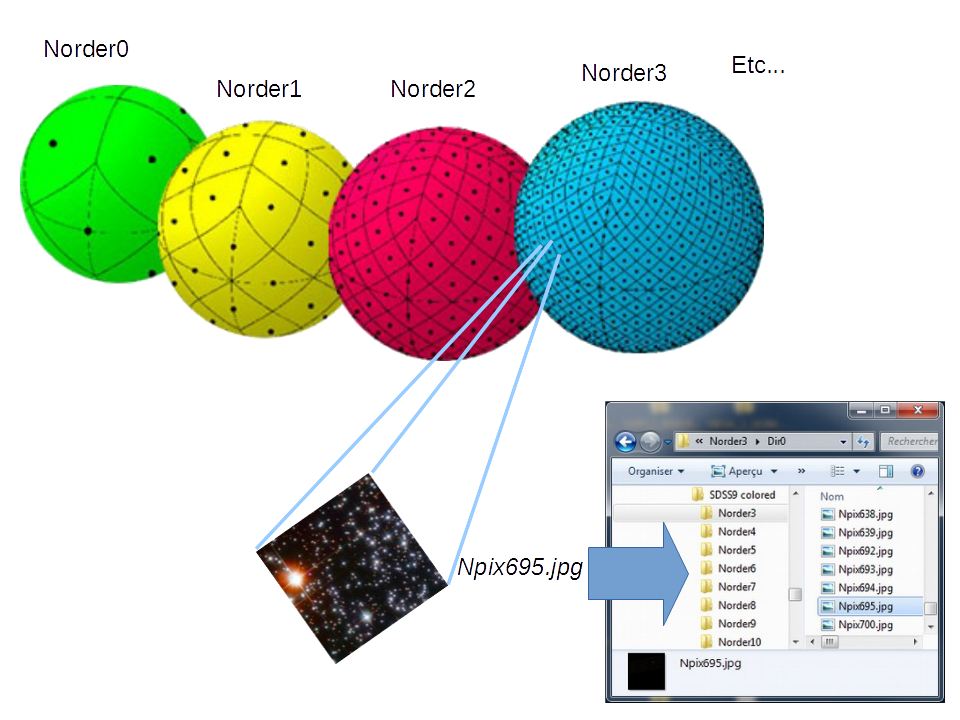
\includegraphics[width=\textwidth]{HiPS-f8.png}
\end{center}
\caption{HiPS architecture based on directories and files}
\label{fig:fig8}
\end{figure}

The number of HiPS orders depends on the original data parameters: the angular resolution for a pixel survey, the number of sources for a catalogue, etc. It also depends on the size of the HiPS tile (see next section). A HiPS may use a partial tree (where not all sphere HEALPix cells are described), notably for a survey that does not cover the whole sky, and it may be possibly not uniform (different depth for different branches) like for catalogue with different densities on the sphere.

\subsubsection{Tile formats}

The content of the HiPS tiles depends on the nature of the original survey: pixel arrays for an image survey, catalogue source list for a catalogue survey, vector arrays for polarization data, properties for localized meta-data (progenitors), etc. This section describes only the format of the tiles dedicated to images and catalogues spatial data respectively to HiPS image and HiPS catalog, The HiPS cube and its related tiles are described in the section \ref{sec:cubicData}.

A HiPS tile must contain the data (pixels, catalogue sources...) located in its associated HEALPix cell on the sky. This implies that the data must have a footprint on celestial sphere (described by a WCS solution for images, and described by spherical coordinates for catalogue sources). The tile format depends on the survey data type: FITS, JPEG, PNG for image; TSV for catalogues. These basic tile formats are not an obligation, but are suggested in order to facilitate checking of the tile content with basic file tools and editors.


\paragraph{HiPS image tile}
\label{sec:shiftOrder}

HiPS image tiles must contain the image pixels located in the associated HEALPix cell. This constraint requires a resampling of the original image pixels into the HEALPix geometry grid (see next section), except for cases where the original data are natively provided in HEALPix (for instance PLANCK data), 

To avoid tiles containing only one HEALPix pixel, HiPS image tile hierarchy is S orders less deep than the original HEALPix resampled data, packaging the $2^{S} \times 2^{S}$ HEALPix cell values, as an array of pixels.

\begin{figure}[h]
\begin{center}
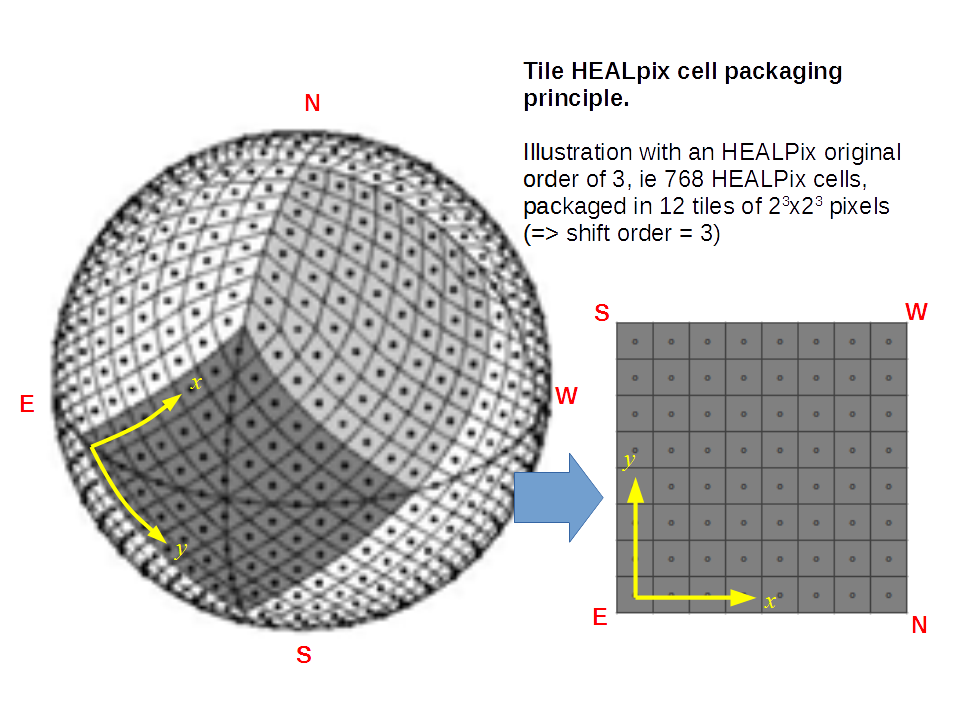
\includegraphics[width=\textwidth]{HiPS-f9.png}
\end{center}
\caption{The HEALPix cell packaging principle in a FITS tile}
\label{fig:fig9}
\end{figure}

\medskip
\noindent\textit{Example: The XMM PN survey (4" pixel angular resolution), requiring a resampling in a HEALPix grid at order 16 (3.221" HEALPix cell angular resolution), may be packaged in HiPS tile at order 7 ($16-9$) containing the $29 \times 29$ HEALPix cell values.}
\medskip

\begin{tcolorbox}
\underline{Best practice: } Because of present capacities of most network infrastructure a tile size of $512 \times 512$ pixels (shift order: S = 9) is a good compromise between the size of the tiles and the number of tiles required to map the original survey data.
\end{tcolorbox}

\paragraph{Deepest HiPS order}

At the deepest HiPS order, the pixels in the tiles are directly computed from the original data. The method for evaluating each pixel value of these tile arrays depends on the HiPS creation algorithm. It may be the nearest pixel, a bilinear interpolation or any other algorithm mapping the original pixels from their original sky grid into the HEALPix grid, and preferably in an ICRS equatorial coordinate system.

Also, in the case of overlapping multiple input original images, an average method, weighted or not, can be applied. This document does not recommend the usage of any specific algorithm.

If the original data come from a native HEALPix map (for instance, PLANCK data), no pixel conversion is then required: each HiPS tile pixel takes the associated HEALPix map cell value. In this case, it would be reasonable to retain the native coordinate system (for instance, galactic in the case of PLANCK data).

The choice of the deepest HiPS order depends on the required HiPS resolution ($\theta$ expressed  in degrees). It may be chosen as the first HEALPix $\textit{order}$ under the original pixel angular resolution. This choice depends on the tile $\textit{width}$ according to this HEALPix function: 


\medskip
\noindent\fbox{%
\parbox{0.98\linewidth}{%
\centering
\[
\theta \approx \frac{360}{2 \pi} \sqrt{ \frac{4 \pi}{12 \times ( \textit{width} \times 2^{\textit{order}} )^{2}} }
\]
}}
\medskip

Thus, the required HiPS \textit{order} is obtained by the reciprocal function:\\
\medskip
\noindent\fbox{%
\parbox{0.98\linewidth}{%
\centering
\[
\textit{order}
=
\log_{2}\!\left(
\frac{360}{2\pi} \times
\;\frac{\sqrt{\pi/3}}{\textit{width}\times \theta}
\right)
\]
}}
\medskip



\begin{longtable}{|l|l|l|l|}
\hline

tile                  & $\theta$ ( pixel          & 512 x 512 tile  & Number  \\ 
order              &  angular size)             & angular size    & of tiles           \\ \hline

0 & 6.871' & 58.63° & 12 \\ \hline
1 & 3.435' & 29.32° & 48 \\ \hline
2 & 1.718' & 14.66° & 192 \\ \hline
3 & 51.53" & 7.329° & 768 \\ \hline
4 & 25.77" & 3.665° & 3072 \\ \hline
5 & 12.88" & 1.832° & 12288 \\ \hline
6 & 6.442" & 54.97' & 49152 \\ \hline
7 & 3.221" & 27.48' & 196608 \\ \hline
8 & 1.61" & 13.74' & 786432 \\ \hline
9 & 805.2mas & 6.871' & 3145728 \\ \hline
10 & 402.6mas & 3.435' & 12582912 \\ \hline
11 & 201.3mas & 1.718' & 50331648 \\ \hline
12 & 100.6mas & 51.53" & 201326592 \\ \hline
13 & 50.32mas & 25.77" & 805306368 \\ \hline
14 & 25.16mas & 12.88" & 3221225472 \\ \hline
15 & 12.58mas & 6.442" & 12884901888 \\ \hline
16 & 6.291mas & 3.221" & 51539607552 \\ \hline
17 & 3.145mas & 1.61" & 2,06158E+11 \\ \hline
18 & 1.573mas & 805.2mas & 8,24634E+11 \\ \hline
19 & 786.3µas & 402.6mas & 3,29853E+12 \\ \hline
20 & 393.2µas & 201.3mas & 1,31941E+13 \\ \hline

\caption{Angular sizes function of the HiPS order with $512 \times 512$ tile size}
\label{tab:tabOrder}
\end{longtable}

\begin{figure}[h]
\begin{center}
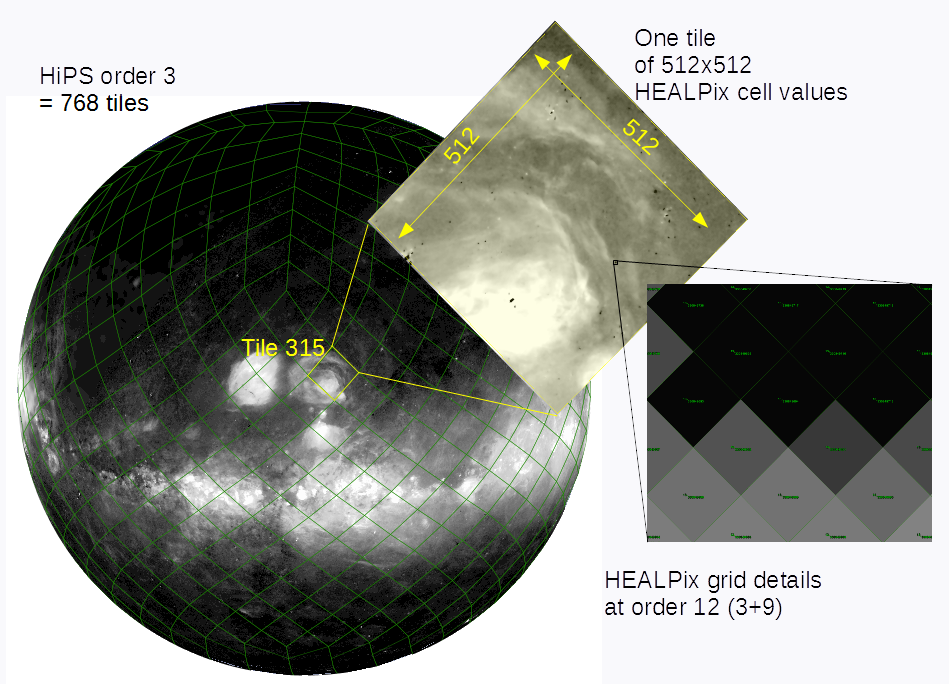
\includegraphics[width=\textwidth]{HiPS-f10.png}
\end{center}
\caption{The HiPS Halpha Finkbeiner survey at HiPS order 3 (768 tiles) with HiPS tiles of $512 \times 512$ HEALPix cell values (51.53" resolution)}
\label{fig:fig10}
\end{figure}

\paragraph{Other HiPS orders}

As explained in the tile structure, there are four times less tiles at order K compared to the order K+1. Each pixel of the tiles at order K is computed from the four pixels at order K+1 covering the same HEALPix area. The method for evaluating this pixel from its 4 sub-pixels depends on the HiPS creation algorithm. It may be the first pixel (one value amongst the 4 values), the mean, the median value, etc. This document does not recommend the usage of any specific algorithm.

\begin{tcolorbox}
\underline{Best practice: } The average method is certainly the most appropriate, particularly when the original pixel values represent a certain intensity per unit area. Alternatively, the median method highlights large-scale structures and reduces the impact of bright stars, while the first pixel method is the fastest.
\end{tcolorbox}

\subparagraph{Format of image tiles}
\label{sec:tileFormat}

Three image formats are suggested in this document to package the HiPS tiles for images: FITS \citep{FITS}, PNG, JPEG. An image tile may be stored in FITS format in order to keep the full dynamic range of the original data values. Tiles stored in JPEG format provide good file compression, and tiles stored in PNG format provides the capability to support transparency channel. The tile file extension must correspond to the format: ".fits" for FITS, ".jpg" for JPEG, ".png" for PNG. These extensions must be in lowercase. Contrary to the FITS convention, in JPEG, and PNG the lines of the pixel array are stored in top $\rightarrow$down direction.

An HiPS image may be delivered simultaneously in various formats. 

\begin{figure}[h]
\begin{center}
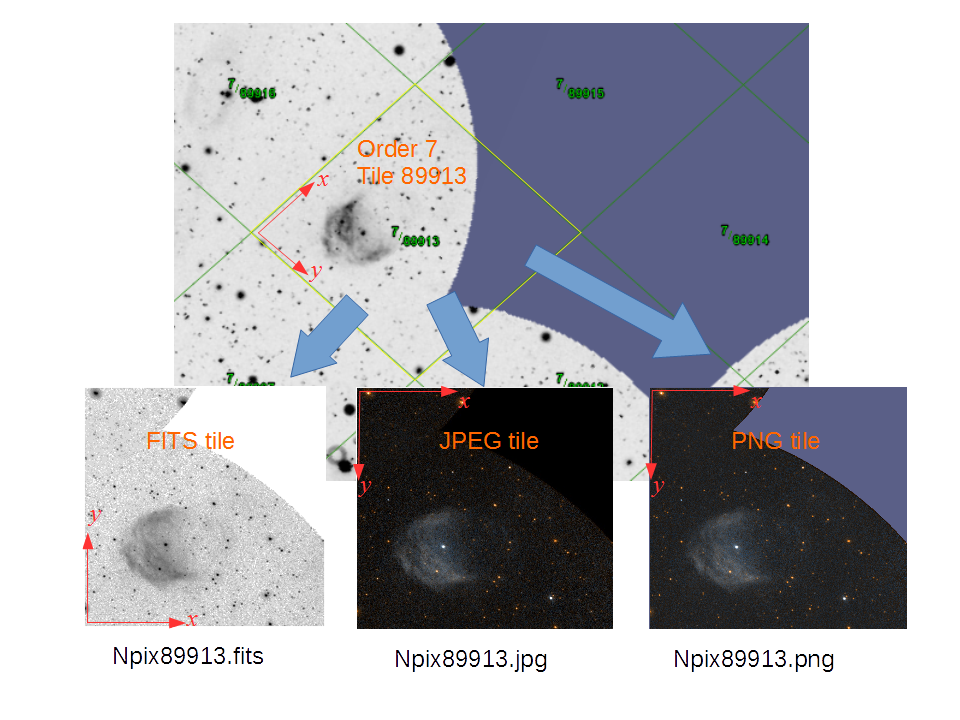
\includegraphics[width=\textwidth]{HiPS-f11.png}
\end{center}
\caption{A GALEX HiPS survey tile provided simultaneously in FITS, JPEG and PNG}
\label{fig:fig11}
\end{figure}

A HiPS can use any another formats if this proves more appropriate, bearing in mind that this will reduce the number of clients able to access such a HiPS. A good example is the RICE FITS compression alternative \citep{Rice1993} or WEBP alternative \citep{RFC9649}. In this last case, it should be prudent  to add rather than replace the collection of tiles in this alternative format \footnote{For the WEBP alternative, the file extension will logically be “.webp.” In the case of RICE FITS, the extension should remain “.fits” because it is a compression mode that does not change the nature of the file since this compression has been integrated into the FITS standard \citep{FITS}.}

% Commentaire Thomas : quelle extension est recommandée pour RICE FITS -> .fits.fz ou .fits ?

\paragraph{HiPS catalog tile}

A HiPS catalog tile must contain a list of catalogue sources corresponding to the original sources located in the associated HEALPix cell.

The distribution of the sources in the HiPS hierarchy may use various algorithms. The most usual method is based on the following principle: if the number of sources in a tile at order K overtakes a threshold, the other sources are stored in the 4 sub-tiles of the order K+1, and so on, recursively. This threshold is not necessary a constant, it may depend of the distribution of the sources, notably for handling the possible local densities. The method for sorting the source may be based on any property of the sources: magnitude, parallax, number of citations…

\begin{tcolorbox}
\underline{Best practice: } A HiPS tile containing a few hundred sources is a good compromise between the size of the tile, the time used to display the information, and the number of tiles required to map the catalogue.
\end{tcolorbox}

The deepest HiPS order for a HiPS catalog is related to the number and the density of the sources and the number of sources stored in each tile.

\subparagraph{Format of catalog tiles}

This document proposes the TSV format for HiPS catalog tiles. As with images, other formats may be considered, despite the fact that there will be potentially fewer compatible clients.

A HiPS catalog TSV tile must be stored in an UTF-8 file (ie ASCII 7 bits + extended characters \citep{RFC3629}) using this TSV convention (Tab Separated Value). The first line is a header providing the column names. All fields, are separated by a TAB (decimal ASCII code 9), and each line is ended by a LF (decimal ASCII code 10), possibly preceded by a CR (decimal ASCII code 13). Any line beginning with a hash (\# - decimal ASCII code 35) is a comment line and it is ignored. An empty field corresponds to the null value (not provided).

All tiles must have the same columns and the same column ordering. Columns providing the location on the sky of each source must be present. The tile file extension must be ".tsv" in lowercase.

\begin{figure}[h]
\begin{center}
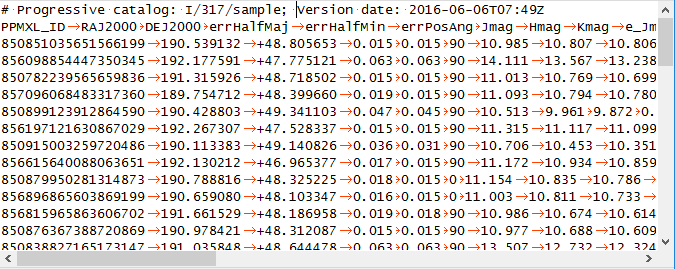
\includegraphics[width=\textwidth]{HiPS-f12.png}
\end{center}
\caption{Excerpt of the HiPS catalog TSV tile Norder5, Npix2741 from PPMXL}
\label{fig:fig12}
\end{figure}


\subsection{Cubic data}
\label{sec:cubicData}

The HiPS method applied to spherical-cubic data, notably for spatio-frequency cubes or spatio-temporal cubes, uses the same discretization principle but simultaneously on the spatial dimension using HEALPix tessellation, and in the additional physical dimension using an ad-hoc discretization function. The generated HiPS tiles will have a depth and will be identified by a unique address composed by the HEALPix cell order and index for the spatial dimension, and by the order and index of the cell resulting from the discretization of the additional physical axis on the other hand.

Consequently, only cubes that are fully calibrated, spatially and in the additional dimension, can give rise to a HiPS cube. 

\begin{figure}[h]
\begin{center}
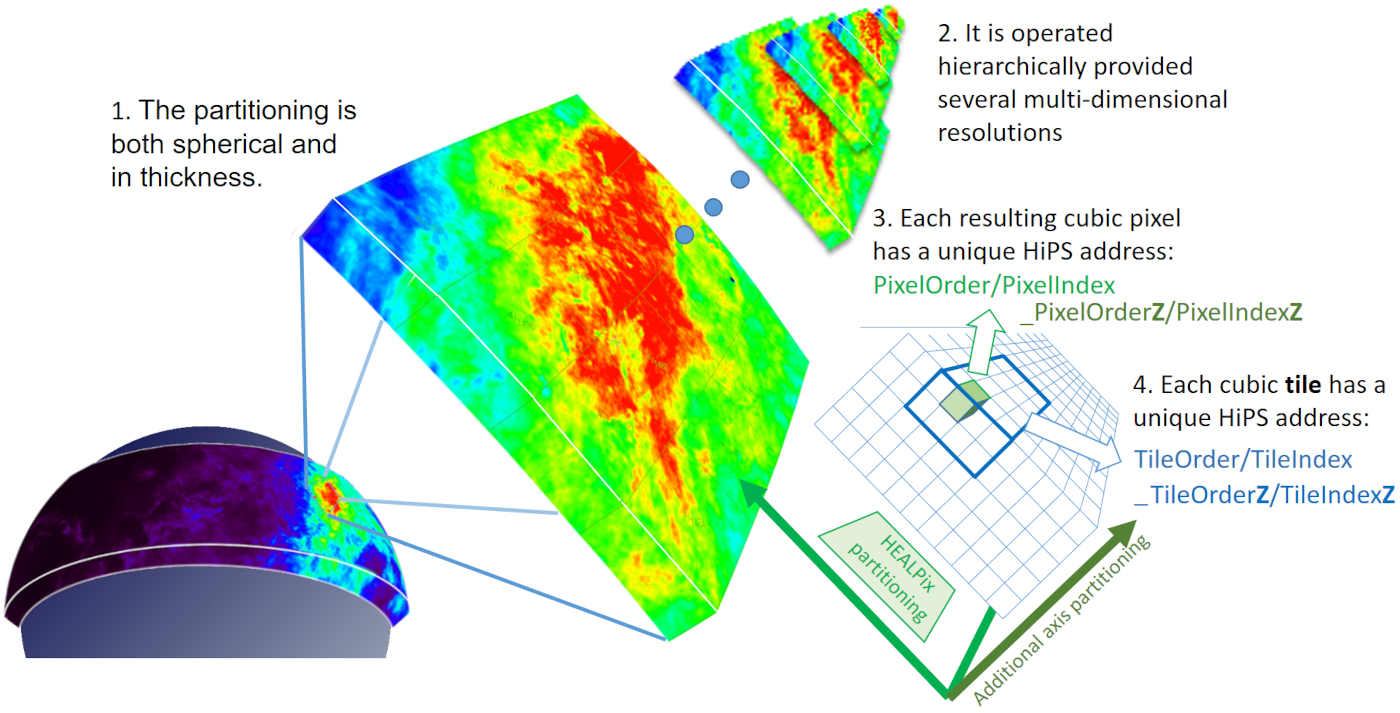
\includegraphics[width=\textwidth]{HiPS-f25.png}
\end{center}
\caption{HiPS spherico-cubicl discretization principle }
\label{fig:fig1}
\end{figure}



Following the same HiPS logic, each cubic pixel within the tiles will be identified by its spatial order and index and by its order and index in the additional physical dimension. Just like tile width, tile depth requires a power of 2. The order gap between the identification of the tile and the identification of a cubic pixel is given by the $log_2$ of the tile width for the spatial dimension, and the $log_2$ of the tile depth for the additional dimension. 

Also, HiPS cube must provide a hierarchy of lower resolution tiles, both in the spatial dimension and in the additional dimension. These tiles are calculated from the higher resolution tiles recursively, starting from the deepest order tiles. Unlike the spatial dimension (2 axes), which reduces the resolution by a factor of 4 with each reduction in order, the additional dimension only concerns a single axis, resulting in a factor of 2 with each reduction in order. Furthermore, the method used to calculate a lower-resolution cubic pixel from its child pixels can be the mean, median, maximum or minimum, one of the values chosen at random, or any other method best suited to the intended use of the HiPS.

As HiPS cube takes two physical dimensions into account simultaneously, it is technically possible to calculate all possible combinations of lower resolution (spatial orders versus additional dimension orders). The choice of combinations depends on the intended use of the generated HiPS (visualization, extraction of sub-cubes, etc.). 

\begin{figure}[h]
\begin{center}
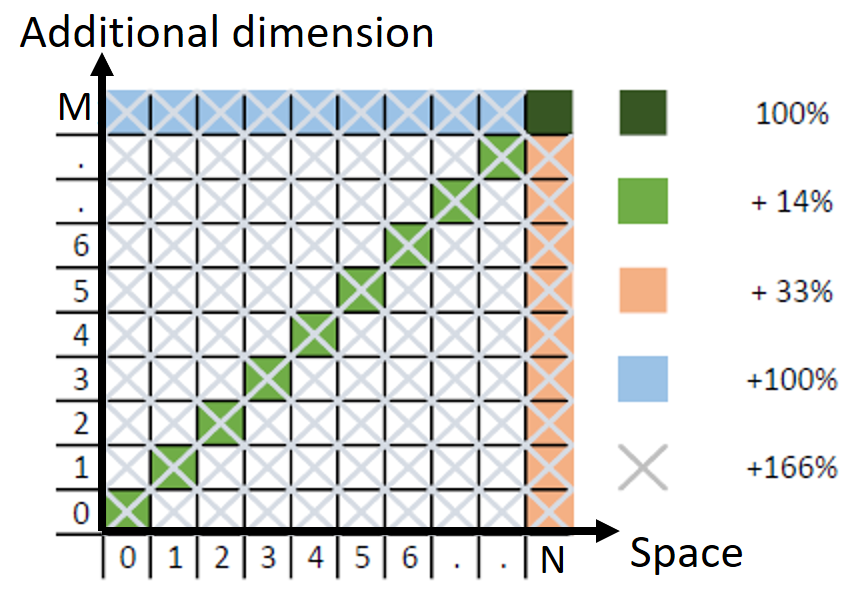
\includegraphics[width=0.6\textwidth]{HiPS-f27.png}
\end{center}
\caption{Combinations of resolution orders: volume costs}
\label{fig:fig27}
\end{figure}

At a minimum, this document recommendes to generate the combination of orders that simultaneously degrade the spatial dimension and the additional dimension represented in color green in the figure \ref{fig:fig27}. Thus, a HiPS cube requiring a spatial order N and an order M for the additional dimension at the best resolution must provide tiles of lower resolution of orders (N-1,M-1), (N-2,M-2), ... up to order 0 for the lower dimension. This minimum recommendation ensures a perfectly satisfactory progressive visualization experience by adding only 14\% of the HiPS volume (8 child cubic pixels for 1 parent cubic pixel) for the lower resolution tiles.

When the respective resolutions in the two physical dimensions are asymmetrical in terms of the deepest order values, it is recommended to add the missing {\bf spatial} orders up to 0, and it may be desirable to do the same in the symmetrical case, but only up to an order that allows the entire coverage to be visualized (not necessary 0). Figure  \ref{fig:fig21} shows the recommended order combinations in dark green and additional desirable combinations in light green. 

\begin{figure}[h]
\begin{center}
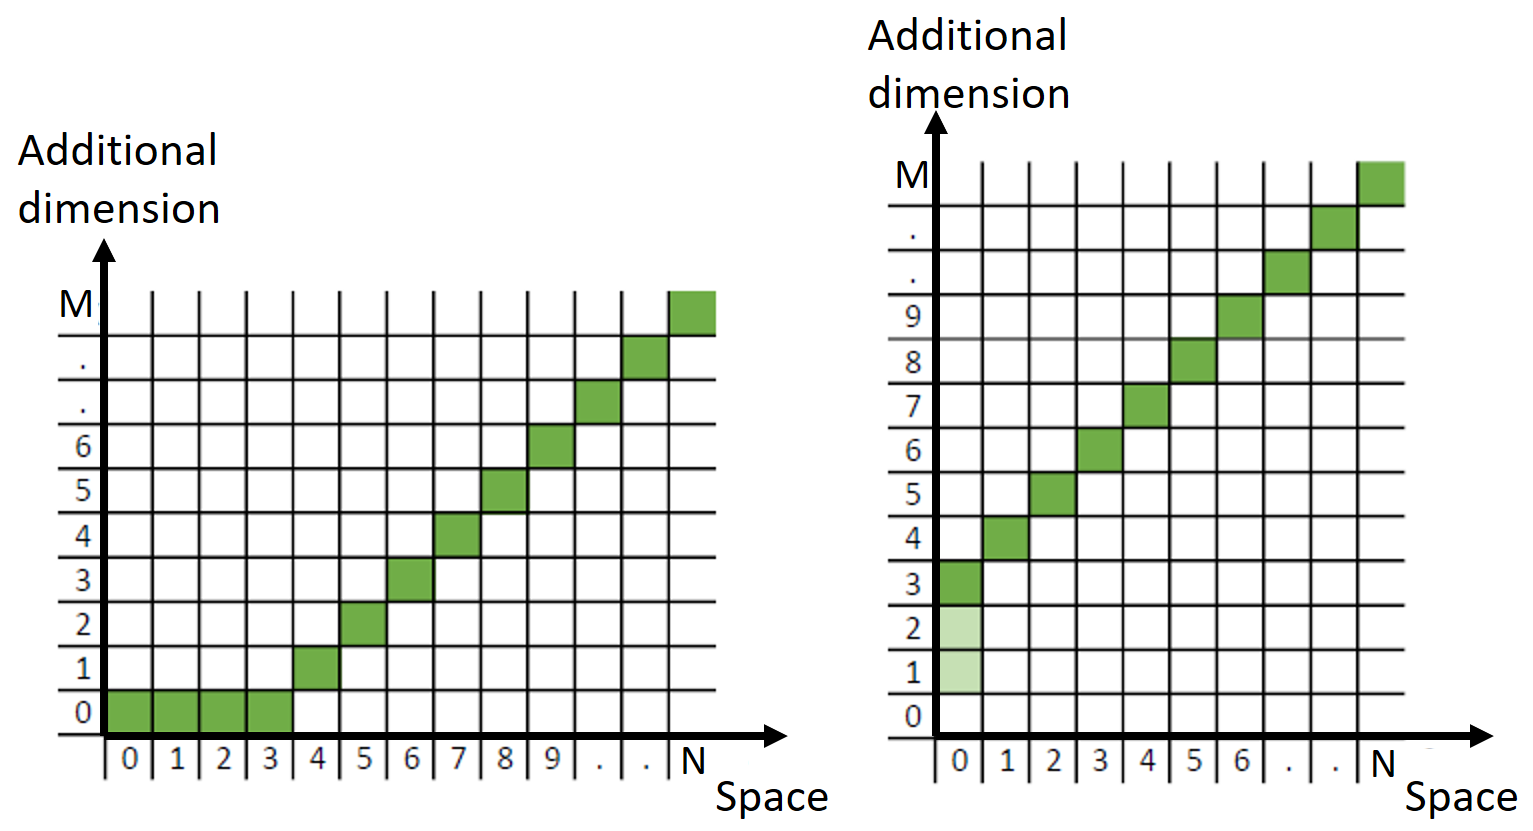
\includegraphics[width=\textwidth]{HiPS-f21.png}
\end{center}
\caption{Combinations of resolution orders: the default choice}
\label{fig:fig21}
\end{figure}

{\em For example, for a spatio-temporal cubic survey requiring a spatial resolution of 12 arcseconds and a temporal resolution of 24 hours, the deepest order tiles will be 5 for the spatial dimension (see  Table \ref{tab:tabOrder}) and 24 for the temporal dimension (see Table \ref{tab:tabOrderTime}). The lowest resolution tiles calculated by default will be (4,23), (3,22), (2,21), (1,20), and (0,19). The HiPS author is free to add any other combinations to this default, for example to continue reducing the temporal orders while maintaining the minimum spatial resolution, such as (0,18), (0,17), and (0,16).}


\subsubsection{Discretization of the additional axis}
This document specifies the recommended functions for temporal discretization as well as frequency discretization. The appendix~\ref{sec:generic} suggestes a generic method for other potential dimensions (altitude, distance, …) but not cover formally by this current HiPS specification.

\paragraph{Temporal discretization}
The discretization function used for time must follow the TMOC convention described in the document MOC 2.1 \citep{MOC2.1}. Any date is expressed as a number in Julian Date Convention in a TCB barycentric reference frame. The time discretization at the maximum resolution (order 61) is performed at the microsecond level and directly provides the time index in this order. 


\medskip
\noindent\fbox{%
\parbox{0.98\linewidth}{%
\centering
\[
\textit{indexT} = \textit{JD} \; \textit{expressed}  \;  \textit{in}  \; \textit{µs}
\]
}}
\medskip


Any time cell of order L and index M covers the same time period as its two daughter cells of order L+1 with indices $M \times 2$ and $M \times 2 +1$, respectively.

\medskip
\noindent\textit{Example:  an observation occurred the January 1th 2000 coded at the order 24 (resolution $\approx$1.6 days) has the the temporal index 1541146, and the index 3082292 at the order 25 (resolution $\approx$19 hours).}
\medskip

The choice of the deepest temporal order depends on the desired resolution and the depth of the HiPS tiles. Table \ref{tab:tabOrderTime} shows the temporal coverage of a tile and of a cell within a tile for each of the possible orders.

\begin{longtable}{|l|l|l||l|l|l|}
\hline
Order & Tile time & Cell time &
Order & Tile time & Cell time \\
       & coverage  & coverage  &
       & coverage  & coverage  \\ \hline
\endfirsthead

\hline
Order & Tile time & Cell time &
Order & Tile time & Cell time \\
       & coverage  & coverage  &
       & coverage  & coverage  \\ \hline
\endhead

0  & $\approx$73067y 276d & $\approx$4566y 268d &
29 & $\approx$1h 11m & $\approx$4m 28s \\ \hline
1  & $\approx$36533y 320d & $\approx$2283y 134d &
30 & $\approx$35m 47s & $\approx$2m 14s \\ \hline
2  & $\approx$18266y 342d & $\approx$1141y 249d &
31 & $\approx$17m 53s & $\approx$1m 7s \\ \hline
3  & $\approx$9133y 171d & $\approx$570y 307d &
32 & $\approx$8m 56s & $\approx$33s 554ms \\ \hline
4  & $\approx$4566y 268d & $\approx$285y 153d &
33 & $\approx$4m 28s & $\approx$16s 777ms \\ \hline
5  & $\approx$2283y 134d & $\approx$142y 259d &
34 & $\approx$2m 14s & $\approx$8s 388ms \\ \hline
6  & $\approx$1141y 249d & $\approx$71y 129d &
35 & $\approx$1m 7s & $\approx$4s 194ms \\ \hline
7  & $\approx$570y 307d & $\approx$35y 247d &
36 & $\approx$33s 554ms & $\approx$2s 97ms \\ \hline
8  & $\approx$285y 153d & $\approx$17y 306d &
37 & $\approx$16s 777ms & $\approx$1s 48ms \\ \hline
9  & $\approx$142y 259d & $\approx$8y 335d &
38 & $\approx$8s 388ms & 524ms 288µs \\ \hline
10 & $\approx$71y 129d & $\approx$4y 167d &
39 & $\approx$4s 194ms & 262ms 144µs \\ \hline
11 & $\approx$35y 247d & $\approx$2y 83d &
40 & 2s 97ms & 131ms 72µs \\ \hline
12 & $\approx$17y 306d & $\approx$1y 41d &
41 & 1s 48ms & 65ms 536µs \\ \hline
13 & $\approx$8y 335d & $\approx$203d 14h &
42 & 524ms 288µs & 32ms 768µs \\ \hline
14 & $\approx$4y 167d & $\approx$101d 19h &
43 & 262ms 144µs & 16ms 384µs \\ \hline
15 & $\approx$2y 83d & $\approx$50d 21h &
44 & 131ms 72µs & 8ms 192µs \\ \hline
16 & $\approx$1y 41d & $\approx$25d 10h &
45 & 65ms 536µs & 4ms 96µs \\ \hline
17 & $\approx$203d 14h & $\approx$12d 17h &
46 & 32ms 768µs & 2ms 48µs \\ \hline
18 & $\approx$101d 19h & $\approx$6d 8h &
47 & 16ms 384µs & 1ms 24µs \\ \hline
19 & $\approx$50d 21h & $\approx$3d 4h &
48 & 8ms 192µs & 512µs \\ \hline
20 & $\approx$25d 10h & $\approx$1d 14h &
49 & 4ms 96µs & 256µs \\ \hline
21 & $\approx$12d 17h & $\approx$19h 5m &
50 & 2ms 48µs & 128µs \\ \hline
22 & $\approx$6d 8h & $\approx$9h 32m &
51 & 1ms 24µs & 64µs \\ \hline
23 & $\approx$3d 4h & $\approx$4h 46m &
52 & 512µs & 32µs \\ \hline
24 & $\approx$1d 14h & $\approx$2h 23m &
53 & 256µs & 16µs \\ \hline
25 & $\approx$19h 5m & $\approx$1h 11m &
54 & 128µs & 8µs \\ \hline
26 & $\approx$9h 32m & $\approx$35m 47s &
55 & 64µs & 4µs \\ \hline
27 & $\approx$4h 46m & $\approx$17m 53s &
56 & 32µs & 2µs \\ \hline
28 & $\approx$2h 23m & $\approx$8m 56s &
57 & 16µs & 1µs \\ \hline


\caption{Tile and cell time coverage function of the order with 16 depth tile }
\label{tab:tabOrderTime}
\end{longtable}

In practical term, the appropriate deepest  ${\textit order}$ required to map a dedicated time resolution ($\Delta t$ expressed in µs) in a tile thickness of {\textit depth} channels will be approximated  by this formulae:\\
\medskip
\noindent\fbox{%
\parbox{0.98\linewidth}{%
\centering
\[
\textit{orderF}
\approx
61
-
\log_{2}\!\bigl(\textit{depth} \times \Delta t\bigr)
\]}}
\medskip

\paragraph{Frequency discretization}
The discretization function used for frequency must follow the FMOC convention described in the document MOC 2.1 \citep{MOC2.1}. Axccording to this document, the frequency must be expressed in Hertz, comprised between $1E-18$ and $1E+38$, and the index for at the maximum resolution (order 51) is based on the following logarithm expression providing a linear normalisation in logarithm space followed by a integer quantification:

\medskip
\noindent\fbox{%
\parbox{0.98\linewidth}{%
\centering
\[
\textit{indexF}
= \left\lfloor \frac{ \log_{10}(\textit{freq}) - \log_{10}(1E-18) }{ \log_{10}(1E+38)-\log_{10}(1E-18) }  \times 2^{52}  \right\rfloor
\]
}}
\medskip

That can be simplified in this expression:\\
\medskip
\noindent\fbox{%
\parbox{0.98\linewidth}{%
\centering
\[
\textit{indexF}
=  \left\lfloor \frac{\log_{10}(\textit{freq}) + 18}{56} \times 2^{52}   \right\rfloor
\]
}}
\medskip

And its reciprocal expression:\\
\medskip
\noindent\fbox{%
\parbox{0.98\linewidth}{%
\centering
\[
\textit{freq}
= 10^{\left(\frac{\textit{indexF} }{2^{52}} \times 56 - 18\right)}
\]
}}
\medskip


Unlike HEALPix and TMOC discretization, FMOC discretization does not maintain equal frequency coverage across channels for a given order. This is due to the logarithmic expression required to cover a large portion of the electromagnetic axis. However, this difference does not change the fundamental principle: any frequency cell of order L and index M covers the same frequency range as its two daughter cells of order L+1 with indices $M \times 2$ and $M \times 2 +1$, respectively.

As with other physical dimensions, the frequency order of HiPS will depend on the desired resolution and tile depth, but also on the frequency band under consideration. Thus the frequency coverage, at a dedicated ${\textit order}$, between to consecutive ${\textit index}$ is provided by this expression:\\
\medskip
\noindent\fbox{%
\parbox{0.98\linewidth}{%
\centering
\[
\Delta \mathrm{freq}
= \mathrm{freq}({\textit indexF})\left(10^{\frac{56}{2^{\textit{orderF}}}} - 1\right)\]
}}
\medskip

%Table \ref{tab:tabBandRes} gives the best average HiPS frequency resolution for a dozen reference frequency bands.
%
%\begin{longtable}{|l|l|l|}
%\hline
%
%Band                        & Band Average        & Resolution      \\
%(UCD categories)     & freq(wavelength)   & at order 51     \\ \hline
%
%em.radio.100-200MHz  & 150MHz(1.999m)       & 8.583µHz(114.353fm)   \\ \hline
%em.radio.6-12GHz     & 10GHz(29.979mm)      & 574.112µHz(1.721fm)   \\ \hline
%em.mm.20-100GHz      & 60GHz(4.997mm)       & 3.441mHz(286.229am)   \\ \hline
%em.mm.750-1500GHz    & 1.125THz(266.482µm)  & 64.453mHz(15.287am)   \\ \hline
%em.IR.30-60µ         & 7.5THz(39.972µm)     & 428.711mHz(2.284am)   \\ \hline
%em.IR.3-4µ           & 87.5THz(3.426µm)     & 5.016Hz(196.512zm)    \\ \hline
%em.opt.R             & 450THz(666.205nm)    & 29.438Hz(43.516zm)    \\ \hline
%em.opt.B             & 675THz(444.137nm)    & 44.125Hz(29.011zm)    \\ \hline
%em.UV.100-200nm      & 2.25PHz(133.241nm)   & 147.25Hz(8.709zm)     \\ \hline
%em.UV.10-50nm        & 18PHz(16.655nm)      & 884Hz(820.563ym)      \\ \hline
%em.X-ray.soft        & 265PHz(1.131nm)      & 17.344kHz(74.033ym)   \\ \hline
%em.X-ray.hard        & 16.5EHz(18.169pm)    & 806.912kHz(888.573rm)  \\ \hline
%em.gamma.soft        & 615EHz(487.467fm)    & 40.108MHz(31.807rm)   \\ \hline
%em.gamma.hard        & 2ZHz(149.896fm)      & 98.304MHz(7.371rm)    \\ \hline
%
%\caption{Best resolution according to frequency band}
%\label{tab:tabBandRes}
%\end{longtable}

In practical term, the appropriate ${\textit order}$ required to map a $ {\Delta f_\text{target}}$ frequency resolution is approximated  by this formulae:\\
\medskip
\noindent\fbox{%
\parbox{0.98\linewidth}{%
\centering
\[
\textit{orderF} \approx \log_2 \left( \frac{56 \cdot \textit{freq}}{\Delta f_\text{target}} \right)
\]
}}
\medskip


\subsubsection{HiPS cube tile and directory structure}

HiPS cube tiles must contain the cubic pixels located in the associated spatio/frequencial (resp. temporal ) cell. This constraint requires a resampling of the original cube pixels into the spherico-cubic geometry (HEALPix and FMOC or HEALPix and TMOC or according to the nature of the cubes).

HiPS cube tiles group adjacent cubic pixels using the same principle as for spatial HiPS (see section~\ref{sec:spatial}). 

The structure of a HiPS cube reused the directories and subdirectories hierarchy (see section~\ref{sec:directory}). They are divided by "order" and "tiles" for both spatial and the additional dimension discretization and an "underscore" (\_) is used for separating both physical dimensions. Thus:

\begin{tcolorbox}
\underline{Best practice: } A tile size of $256 \times 256 \times 16$ is a good compromise to provide good time access. This corresponds to a shift order of 8 on the spatial dimension (see section~\ref{sec:shiftOrder}) and 4 for the additionnal dimension.
\end{tcolorbox}

\medskip
\noindent\fbox{%
\parbox{0.98\linewidth}{%
\begin{center}
Tile N/ K\_M/L
 $\rightarrow$ \texttt{…/NorderK\_L/DirD\_E/NpixN\_M\{.ext\}}
\end{center}
where K is the spatial order, L the additional dimension order, \\
N the tile's HiPS spatial index (HEALPix method), M the tile's additional dimension index.\\
 $D = \lfloor N//10000 \rfloor \times 10000$ and $E= \lfloor M//10  \rfloor \times 10$, \\
and \texttt{\{.ext\}} depends on the nature of the survey (see ``tile format'' below).
}}
\medskip


\begin{figure}[h]
\begin{center}
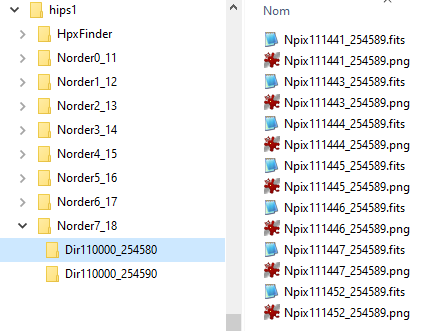
\includegraphics[width=0.7\textwidth]{HiPS-f15.png}
\end{center}
\caption{Directory structure of a HiPS cube}
\label{fig:fig15}
\end{figure}

This method allows any combination "NorderX\_Y" to be taken into account corresponding to a spatial resolution versus a resolution of the additional axis (time or frequency).

\subsubsection{Cubic tile formats}

HiPS cube tiles are cubes of pixels stored in the appropriate directories (see below). The suggested formats are FITS for fully dynamic pixel value tiles, PNG or JPEG for compressed tiles. 

\paragraph{Full dynamic tiles}
The full dynamic tiles use the FITS format for cube arrays following the FITS convention.

\paragraph{Compressed tiles}
%In the case of compressed tiles, the choice is based on classic image compression PNG, JPEG but using a "column" arrangement. The cube is stored "flat" in one column, and n rows corresponding to the number of slices of the cubic tiles. For each slice, the pixel ordering follows the spatial HiPS convention for compressed tiles (see section~\ref{sec:tileFormat}).

 In the case of compressed tiles, the choice is based on classic image compression PNG, JPEG but using a "checkerboard" arrangement.  The cube is stored in lines and column. The number of columns is the square root of the number of channels, rounded down to the lowest integer (e.g.: a 32-channel tile will be stored on a $5 \times 7$ checkerboard). 

\begin{figure}[h]
\begin{center}
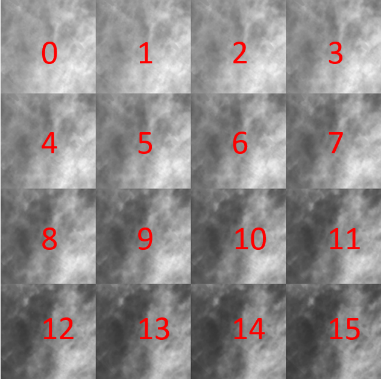
\includegraphics[width=0.6\textwidth]{HiPS-f16.png}
\end{center}
\caption{Example of a checkerboard arrangement of a 16-channel compressed HiPS cube tile}
\label{fig:fig16}
\end{figure}

\subsection{HiPS "enablers"}

This section presents optional "enablers" that can be implemented when generating HiPS to make them easier to use. They enable faster processing and consume fewer resources. It is up to the client to verify whether or not these "enablers" have been implemented.

\subsubsection{WCS solution for FITS tiles}
\label{sec:WCS}

Although each tile, thanks to its HiPS address based on order and index, is perfectly located spatially on the sphere, it may be useful to add the spatial calibration WCS corresponding to this location in the header of the FITS tiles, following the FITS convention for HEALPIX (HPX) projection (FITS reference + Calabretta paper). This way, any FITS manipulation tool, even outside the HiPS context, will be able to spatially manipulate these HiPS FITS tiles.

\medskip
\noindent\textit{For example: the HiPS tile order 0, index 7, and size $512 \times 512$ pixels may contain the following WCS keywords in its header:}
\begin{verbatim}
      CTYPE1  = 'RA---HPX'
      CTYPE2  = 'DEC--HPX'
      CRPIX1  = -255.5
      CRPIX2  = -255.5
      CRVAL1  = 0
      CRVAL2  = 0
      CD1_1   = -8.7890625E-02
      CD1_2   = -8.7890625E-02
      CD2_1   =  8.7890625E-02
      CD2_2   = -8.7890625E-02
      PV2_1   = 4
      PV2_2   = 3
\end{verbatim}
\medskip

Similarly in the case of a HiPS cube, it may be helpful to insert the WCS solution of the additional dimension. The dedicated WCS keywords and associated methods for filling them in are listed in Appendix~\ref{sec:cubicFormula} for the frequency case and for the time case.

\subsubsection{Trim reduction for FITS tiles}

A "trim" operation may be applied on FITS tiles to avoid storing and transporting BLANK, or NaN values for areas not concerned by the survey. If applied, the FITS header uses the keywords TRIM1, TRIM2 to indicate the size of the unstored margins. For each of the axes concerned, the values associated with the NAXIS1 and NAXIS2 keywords will be adjusted to the size of the stored matrix (without the initial and final margins), and the original size of the cube will be saved using the ONAXIS1 and ONAXIS2 keywords. To manipulate such a tile, it will therefore be necessary to identify the presence or absence of the TRIM keywords, and to enlarge the matrix size accordingly, filling the margins created by the BLANK value (resp. NaN for not integer values). 

\begin{figure}[h]
\begin{center}
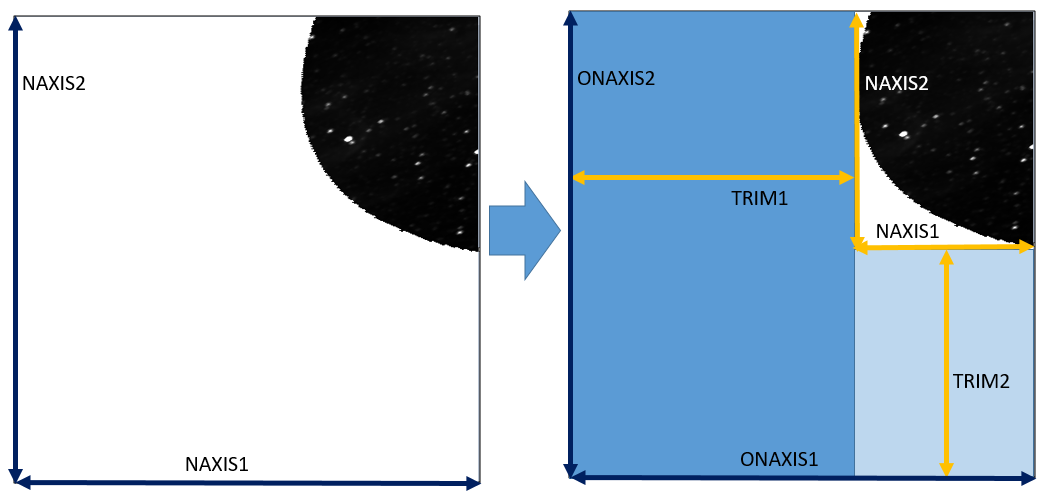
\includegraphics[width=0.9\textwidth]{HiPS-f23.png}
\end{center}
\caption{"Trim" operation to a FITS tile}
\label{fig:fig23}
\end{figure}

As for spatial FITS tile, a"trim" operation may be applied on cubic FITS tile thanks to the FITS keyword TRIM3 and ONAXIS3 in addition to TRIM1, TRIM2 and ONAXIS1, ONAXIS2. 

This operation is particularly effective in terms of volume saved on HiPS built from pointed observations, where the "empty" margins can be significant, especially in low-resolution tiles of the HiPS hierarchy, and this gain will be logically greater for HiPS cubes. Unlike traditional compression algorithms such as GZIP or RICE, this method is trivial and does not add any additional processing time, either for writing or reading. Plus, it retains direct pixel access property.

\underline{Note:} The WCS calibration possibly stored in the tile header (see section~\ref{sec:WCS} above) must take into account the eventual removal of margins. If this calibration is to be used to manipulate the tile, it will be necessary to adjust the position of the calibration reference pixel by adding the values TRIM.

%\subsubsection{Low resolution "enablers"}
%
%The drawing of the lowest HiPS orders that correspond to large sky regions (>30 deg) can be difficult because of:
%\begin{itemize}[noitemsep,topsep=0pt,parsep=0pt,partopsep=0pt]
%\item the high level of distortion of these tiles when a basic/fast 4 corners bilinear drawing method is used (see section 6).
%\item the large number of tiles required for drawing large regions, even at low HiPS order.
%\end{itemize}
%
%In case of spatial HiPS (not applicable for cubix HiPS), to easy the client drawing process, two other enablers may be implemented: order omission and Allsky preview
%
%\subparagraph{Order omission}
%The low orders: order 0 (12 tiles), order 1 (48 tiles), order 2 (192 tiles) may be simply omitted, meaning that the survey files are not provided at these low resolutions.
%
%\subparagraph{Allsky preview file}

\subsubsection{"Allsky" file}
For spatial HiPS, and only for spatial HiPS, the tiles at low orders (0 to 3) may be packaged together into a unique file called Allsky. These files must be located in the NorderK corresponding directory (where K is between 0 and 3). The associated regular tiles must not be removed, notably for supporting basic HiPS clients. The method to generate the Allsky file depends on the nature of surveys:
\begin{itemize}

\item HiPS image Allsky: The Allsky file is built as an array of tiles, stored side by side in the left-to-right order. The width of this array must be the square root of the number of the tiles of the order. For instance, the width of this array at order 3 is 27 ( (int)sqrt(768) ). To avoid having a too large Allsky file, the resolution of each tile may be reduced but must stay a power of two (typically 64x64 pixels rather than 512x512).
\begin{figure}[h]
\begin{center}
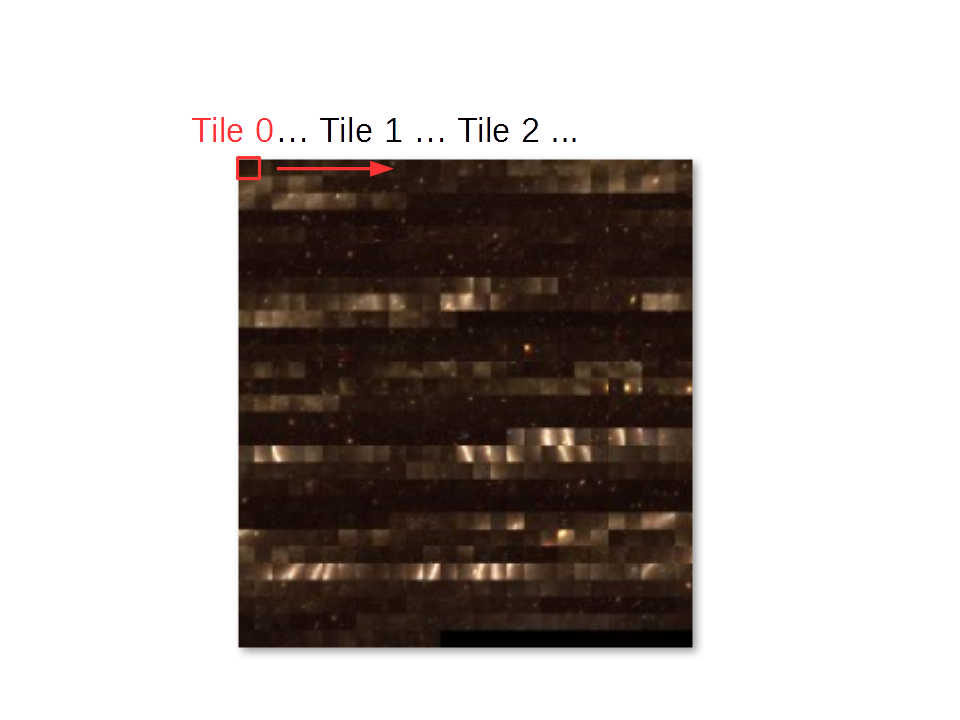
\includegraphics[width=\textwidth]{HiPS-f13.png}
\end{center}
\caption{Example of HiPS Fermi color Allsky.jpg file}
\label{fig:fig13}
\end{figure}

\item HiPS catalog Allsky: The Allsky file is built as the concatenation of all the catalogue tiles. 
\end{itemize}


\subsection{HiPS metadata}

Five additional files must, should or may be used for specifying survey metadata:
\begin{enumerate}[noitemsep,topsep=0pt,parsep=0pt,partopsep=0pt]
\item the properties file (required);
\item the Moc.fits file;
\item the metadata file (recommended under condition);
\item the preview.jpg file (optional);
\item the index.html file (optional).
\end{enumerate}

\subsubsection{The properties file}

A text file named properties must be provided. It specifies generic meta information such as identification, description, copyright, creation date, pixel range, etc.

This properties file must be located in the HiPS root directory. It must be coded in UTF-8 (ie ASCII 7 bits + extended characters \citep{RFC3629}), one line per property, following the syntax keyword = value. Each line is ended by LF (decimal ASCII code 10), possibly preceded by CR (decimal ASCII code 13). Lines starting with a hash as first character (decimal ASCII code 35) must be ignored as comment line. Blank lines must be ignored. Key word cannot include the character "=" (decimal ASCII code 61) or spaces (blank, TAB, ..), and the possible spaces before and after the character "=" must be ignored. The ordering of the keywords is not important. The number of characters in values is not limited.

\begin{tcolorbox}[title=Example of a properties file for HiPS image]
\begin{verbatim}
creator_did          = ivo://SSC/P/XMM/EPIC
obs_collection       = XMM-Newton
obs_title            = XMM-Newton stacked EPIC images
obs_ack              = HE-Team (Strasbourg), SSC XMM-Newton
obs_copyright        = (c) ESA / SSC XMM-Newton
t_min                = 51577.46
t_max                = 56331.92
obs_regime           = X-ray
em_min               = 1e-10
em_max               = 6e-9
dataproduct_type     = image
hips_creation_date   = 2025-10-01T14:07Z
hips_builder         = Aladin/HipsGen v12.650
hips_version         = 1.5
hips_release_date    = 2025-10-05T08:46Z
hips_publisher       = SSC XMM-Newton
hips_frame           = equatorial
hips_order           = 7
hips_tile_width      = 512
hips_status          = public master clonable
hips_tile_format     = png fits
hips_pixel_bitpix    = 32
hips_pixel_cut       = 0 50.95
\end{verbatim}
\end{tcolorbox}

\medskip

\begin{tcolorbox}[title=Example of properties key words dedicated\\to frequency-spacial HiPS cube]
\begin{verbatim}
dataproduct_type     = spectral-cube
hips_order           = 4
hips_order_axis2     = 17
hips_order_hierarchy = 4_17 3_16 2_15 1_14 0_13 0_12 0_11
hips_tile_width      = 256
hips_tile_depth      = 16
obs_restfreq         = 1.420405751E9
\end{verbatim}
%\caption{Example of a properties file for HiPS cube}
\end{tcolorbox}

\underline{Note:} The keyword vocabulary re-uses as far as possible the ObsCore IVOA vocabulary and syntax \citep{2017ivoa.spec.0509L}. 

\medskip

There are 9 mandatory keywords which must be specified:
\begin{enumerate}[noitemsep,topsep=0pt,parsep=0pt,partopsep=0pt]
\item {\bf creator\_did:}  Unique identifier of the HiPS – Format: IVOID \citep{2016ivoa.spec.0523D} – e.g.: ivo://CDS/P/2MASS/J
\item {\bf obs\_title}: Data set title – Format: free text, but should be short (no more than one line) – e.g.: HST 110W
\item {\bf dataproduct\_type:} Type of data – Format: word "image", "catalog", "spectral-cube", "time-cube" respectively for HiPS image, HiPS catalog, spectral and temporal HiPS cube.
\item {\bf hips\_version:} HiPS version number – Format: word "1.5" corresponds to this document specification.
\item {\bf hips\_release\_date}: HiPS release date – Format: ISO 8601 (YYYY-mm-ddTHH:MMZ)
\item {\bf hips\_status}: HiPS status description – Format: list of blank separated words ("private" or "public"), ("master", "mirror", or "partial"), ("clonable", "unclonable" or "clonableOnce"\footnote{"clonableOnce" implies that the copy is allowed, but only from the "master" site} ) – Default : public master clonableOnce
\item {\bf hips\_tile\_format}: Tile formats – Format: list of different HIPS tiles format supported by the survey, space separated (one or many of "fits", "jpeg", "png" for image/HiPS cube and "tsv" for HiPS catalog)
%\item {\bf hip\_order:} Deepest HiPS order(s) – Format: integer (suffixed by \_integer in case of HiPS cube)
\item {\bf hip\_order:} Deepest spatial HiPS order – Format: integer
\item {\bf hips\_frame:} Coordinate frame reference – Format: "equatorial" (ICRS), "galactic", "ecliptic", plus body frame (planeto HiPS) according to the used HiPS coordinate reference.
\end{enumerate}

\medskip
There are 4 additional mandatory keywords specific to the type of HiPS, and they must be specified in the following cases:
\begin{enumerate}[noitemsep,topsep=0pt,parsep=0pt,partopsep=0pt]
\item {\bf dataproduct\_subtype:} Subtype of data – Format: word "color", "live" respectively for HiPS image colored (based on colored tiles), and live HiPS (HiPS for which the content may evolve – for instance live databases like Simbad, or observation missions still in progress)
\item {\bf hip\_order\_axis2:} Dedicated to HiPS cubes, deepest HiPS order for the additional dimension – Format: integer
\item {\bf hips\_order\_hierarchy:}  Explicit list of provided orders in case of divergence with the default recommendation – Format: integer[\_integer] integer[\_integer] ... 
\item {\bf hips\_body:}  Name of the body (dedicated to planetary HiPS – Format: lowercase word  "mercury", "venus", "earth", "mars", "saturn", "jupiter","uranus", "neptun", "pluto", "sun", "moon", "titan", "io", etc.
\end{enumerate}

\medskip
Other keywords should or may be specified. 

The list in the tables below is not exhaustive and new keywords may be added if required. The vocabulary associated to some keywords are not exhaustive and may be extended if required. Some keywords may be repeated to specify multiple values like provenance. The first table contains technical keywords used for HiPS clients, and the second table contains descriptive keywords.

(*) The second column indicates the status of the keyword: *-possibly repeated, R-required, S-should,  D-deprecated (still supported but replaced by another keyword), [] under specific conditions.

\begin{longtable}{|l|c|l|}
\hline
{\bf Technical key word} & (*)  & {\bf Description – Format – Example}  \\ \hline
\endfirsthead
%\hline
%{\bf Key word} & (*)  & {\bf Description – Format – Example}  \\ \hline
%\endhead

creator\_did & R & Unique ID of the HiPS - Format: IVOID\\ & & - Ex : ivo://CDS/P/2MASS/J \\ \hline
hips\_release\_date & R & Last HiPS update date\\ & & - Format: ISO 8601 => YYYY-mm-ddTHH:MMZ \\ \hline
hips\_version & R & Number of HiPS version\\ & & – Format: 1.5 (corresponds to this document) \\ \hline
hips\_service\_url &  & HiPS access url (dedicated to HiPS list - see \Ref{sec:hipslist})\\ & &  – Format: URL \\ \hline
hips\_status & R & HiPS status – Format: list of blank\\ & & separated words (private" or "public"), \\
 & & ("master", "mirror", or "partial"), ("clonable",\\ & & "unclonable" or "clonableOnce") \\
 & &  – Default : public master clonableOnce \\ \hline
hips\_frame & R & Coordinate frame reference – Format: word\\ & & "equatorial" (ICRS), "galactic", "ecliptic", body frame... \\ \hline
hips\_body & [R] & Planet name - Format: lowercase word - Ex: "mercury" \\ \hline
%hips\_order & R & Deepest HiPS order(s) \\ & & – Format: int (HiPS cube: int\_int) \\ \hline
hips\_order & R & Deepest spatial HiPS order – Format: int \\ \hline
hips\_order\_axis2 & R & Deepest HiPS cube second axis \\ & & – Format: int \\ \hline
hips\_order\_min & D & Lowest HiPS order - use hips\_order\_hierarchy instead\\ & & – Format: integer – Default: 0 \\ \hline
hips\_order\_hierarchy & [R] &  Explicit list of orders \\ & & – Format: int[\_int] int[\_int] ... \\ \hline
hips\_tile\_width & R & Tiles width in pixels – Format: positive integer\\ & & – Default : 512, 256 for cubes \\ \hline
hips\_tile\_depth & R & Tiles depth (HiPS cube) – Format: positive integer\\ & & – Default : 16 \\ \hline
hips\_tile\_format & R & List of available tile formats.\\ & & The first one is the default suggested to the client \\
 & &  – Format: list of word blank separated:\\ & &  "jpeg", "png", "fits", "tsv" \\ \hline
dataproduct\_type & R & Type of data – Format: word "image",\\ & & "catalog", "spectral-cube", "time-cube" \\ \hline
dataproduct\_subtype & [R] & Subtype of data – Format: word "color", "live" \\ \hline
hips\_pixel\_cut &   & Suggested pixel display cut range\\ & & (physical values) – Format: min max – Ex : 10 300 \\ \hline
hips\_bunit & S  & pixel physical unit – Format: string \\ \hline
hips\_initial\_ra & S  & Default RA display position (see hips\_initial) \\ & & – Format: real (ICRS frame)  – Unit: degrees \\ \hline
hips\_initial\_dec & S & Default DEC display position (see hips\_initial )\\ & & – Format: real (ICRS frame) – Unit: degrees \\ \hline
hips\_initial\_fov & S & Default display size(see hips\_initial) \\ & &  – Format: real – Unit : degrees \\ \hline
hips\_initial\_freq & S & Default frequency display position \\
 &   & – Format: integer – Unit : Hertz  \\ \hline
hips\_initial\_time & S & Default date display \\
 &   &  –  Format: ISO8601  => YYYY-mm-ddTHH:MMZ \\ \hline
hips\_progenitor\_url &   & URL to an associated progenitor HiPS \\ \hline

\caption{HiPS property keywords -Technical part}
\label{tab:keywords}
\end{longtable}


\begin{longtable}{|l|c|l|}
\hline
{\bf Descriptive key word} & (*)  & {\bf Description – Format – Example}  \\ \hline
\endfirsthead
%\hline
%{\bf Key word} & (*)  & {\bf Description – Format – Example}  \\ \hline
%\endhead

publisher\_id &   & Unique ID of the HiPS publisher\\ & & – Format: IVOID - Ex : ivo://CDS \\ \hline
obs\_collection &   & Short name of original data set\\ & & – Format: one word – Ex : 2MASS \\ \hline
obs\_title & R & Data set title – Format: free text, one line\\ & & – Ex : HST F110W observations \\ \hline
obs\_description & S & Data set description\\ & & – Format: free text, longer free text\\ & & description of the dataset \\ \hline
obs\_ack &   & Acknowledgment mention. \\ \hline
prov\_progenitor (*) & S & Provenance of the original data – Format: free text \\ \hline
bib\_reference & * & Bibliographic reference (bibcode, DOI, arXiv, etc)\\ & &   – Ex: 2015A\&A...576A.135G,10.4225/41/593620ad5b574,\\ & &   arXiv:2503.14451\\ \hline
bib\_reference\_url & *  & URL to bibliographic reference \\ \hline
obs\_copyright &   & Copyright mention associated to the original data\\ & & – Format: free text \\ \hline
obs\_copyright\_url &   & URL to a copyright mention \\ \hline
hips\_copyright &  & Copyright mention associated to the HiPS\\ & & – Format: free text \\ \hline
hips\_licence & [S] & HiPS licence – Format: machine readable licence mention\\ 
 & &  or free text if not applicable – Ex: CC-by-sa\\ \hline
hips\_doi &   & HiPS DOI – Format: DOI syntax\\ 
 & &   – Ex: 10.26093/cds/aladin/pg0c-rj\\ \hline
obs\_regime (*) & [S] & General wavelength\\ & & – Format: word: "Radio" | "Millimeter" | "Infrared"\\
 & & | "Optical" | "UV" | "EUV" | "X-ray" | "Gamma-ray" \\ \hline
data\_ucd (*) &   & UCD describing data contents \\ \hline
hips\_builder &   & Name and version of the tool used for building the HiPS\\ & & – Format: free text \\ \hline
hips\_processing &   & HiPS data processing steps description (calibration, \\ & & transformation, combination, etc). – Format: free text \\ \hline
hips\_history & * & Textual description of the processing history of the HiPS,\\ & &  for creation and updates. (including corresponding dates)\\ & &  – Format: free text \\ \hline
hips\_creator &  S  & Institute or person who built the HiPS\\ & & – Format: free text – Ex : CDS (T.Boch) \\ \hline
hips\_creation\_date & S & HiPS first creation date\\ & & - Format: ISO 8601 => YYYY-mm-ddTHH:MMZ \\ \hline
hips\_data\_minmax &   & HiPS pixel data range\\ & & (physical values) – Format: min max – Ex : 1 4000 \\ \hline
%hips\_data\_range &   & Pixel data range taken into account\\ & &t during the HiPS generation (physical values)\\
% & &  – Format: min max – Ex : -18.5 510.5 \\ \hline
hips\_sampling &   & Sampling applied for the HiPS generation\\ & & – Format: words "none", "nearest", "bilinear" \\ \hline
hips\_overlay &   & Pixel composition method applied\\ & & on the image overlay region during HiPS generation\\
 & & – Format: strings \\ \hline
hips\_skyval &   & Sky background subtraction method applied\\ & &  during HiPS generation – Format: word: \\
 & & "none", "hips\_estimation", "fits\_keyword" \\ \hline
hips\_pixel\_bitpix &   & Fits tile BITPIX code\\ & & – Format: -64, -32, 8, 16, 32, 64 (FITS convention) \\ \hline
%data\_pixel\_bitpix &   & Original data BITPIX code\\ & &  - Format: -64, -32, 8, 16, 32, 64 (FITS convention) \\ \hline
hips\_cat\_nrows & S & Number of rows of the HiPS catalog\\ & & – Format: positive integer \\ \hline
hips\_estsize &   & HiPS size estimation\\ & &  – Format: positive integer – Unit : KB \\ \hline
hips\_nb\_tiles &   & Number of HiPS tiles (all formats)\\ & &  – Format: positive integer \\ \hline
%data\_cube\_bunit3 &   & Third axis unit (see FITS doc) – Format: string \\ \hline
%hips\_initial\_display & S & Initial display coverage – Format: ASCII MOC cell\\ & & – ex: s10/12455 f34/60202 \\ \hline
obs\_restfreq &   & Reference frequency for HiPS cube visualize in speed\\ & & - Format: real - Unit: Hertz \\ \hline
hips\_pixel\_scale &   & HiPS pixel angular resolution at the highest order\\ & & – Format: real – Unit : degrees \\ \hline
%s\_pixel\_scale &   & Best pixel angular resolution of the original images\\ & & – Format: real – Unit : degrees \\ \hline
t\_min & S & Start time of the observations – Format: real\\ & & – Representation: MJD  \\ \hline 
t\_max & S & Stop time of the observations – Format: real \\ & & – Representation: MJD \\ \hline
em\_min & S & Start in spectral coordinates – Format: real \\ & & – Unit: meters \\ \hline
em\_max & S & Stop in spectral coordinates – Format: real \\ & & – Unit: meters \\ \hline
client\_category &   & '/' separated keywords suggesting a display \\ & & hierarchy to the client – Ex : Image/InfraRed \\ \hline
client\_link & *  & ID of related HiPS  - Format: IVOID\\ & & - Ex: ivo:CDS/P/Simbad\_density\_map \\ \hline
%client\_sort\_key &   & Sort key suggesting a display order to\\ & & the client inside a "client\_category"\\
% & & – Format: free text – Sort : alphanumeric \\ \hline
%addendum\_did & *  & In case of "live" HiPS, creator\_did of the added HiPS \\ \hline
moc\_sky\_fraction &   & Fraction of the sky covers by the MOC\\ & & associated to the HiPS – Format: real between 0 and 1 \\ \hline

\caption{HiPS property keywords - Descriptive part}
\label{tab:keywords1}
\end{longtable}



\subsubsection{The Moc.fits file}

A file named Moc.fits, located in the HiPS root directory, should be provided. It represents the coverage map of the HiPS tiles. This file follows the IVOA MOC document \citep{MOC2.1}. The client can use it as a summary of the coverage of the HiPS to avoid trying to load tiles outside the coverage area of the HiPS.
For a HiPS cube, this MOC file will be an STMOC for spatio-temporal coverage, or an SFMOC for spatio-frequency coverage.

The MOC provided must necessarily be in the same reference frame(s) as the HiPS, notably for HiPS of a planetory surface or celestial galactic HiPS.

\subsubsection{The metadata file}

In addition to the generic metadata described in the properties file (see 4.4.1), a file called metadata.xxx, located in the HiPS root directory may be provided for specific meta information such as column descriptions, original FITS keywords, etc. This information depends on the survey data type:
\begin{itemize}
\item {\bf HiPS image metadata}: the metadata are stored as a FITS header (FITS convention) in metadata.fits file for providing generic FITS header keywords. This file can be reduced to a FITS header or even a regular FITS file from the original survey containing the FITS header used for global metadata information – in the second case the image array is simply ignored by the client.
\item {\bf HiPS catalog metadata}: the metadata are stored in metadata.xml file as a fully defined VOTable (column descriptions, units, ucds,...) \citep{2019ivoa.spec.1021O}. All column information associated with the source tiles must be provided via the "metadata" file. The internal header of each individual tile is ignored by the client (VOTable metadata richer than the default simple header line, notably for designating columns containing the spatial locations).
\item {\bf HiPS cube metadata}: same as for HiPS image.
\end{itemize}

\subsubsection{The preview.jpg file}

A file called preview.jpg, located in the HiPS root directory may be provided to offer a preview of the HiPS. This image is $256 \times 256$ pixel size, stored in JPEG format.

\begin{figure}[h]
\begin{center}
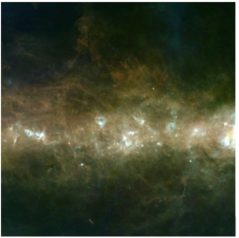
\includegraphics[width=0.4\textwidth]{HiPS-f17.png}
\end{center}
\caption{preview.jpg file associated to the AKARI colored HiPS}
\label{fig:fig17}
\end{figure}

\subsubsection{The index.html file}

A file called index.html, located in the HiPS root directory may be provided to offer a simple HTML presentation of the survey. By loading the root HiPS directory location one will be able to display information about the HiPS itself through any Web browser. 

\begin{figure}[h]
\begin{center}
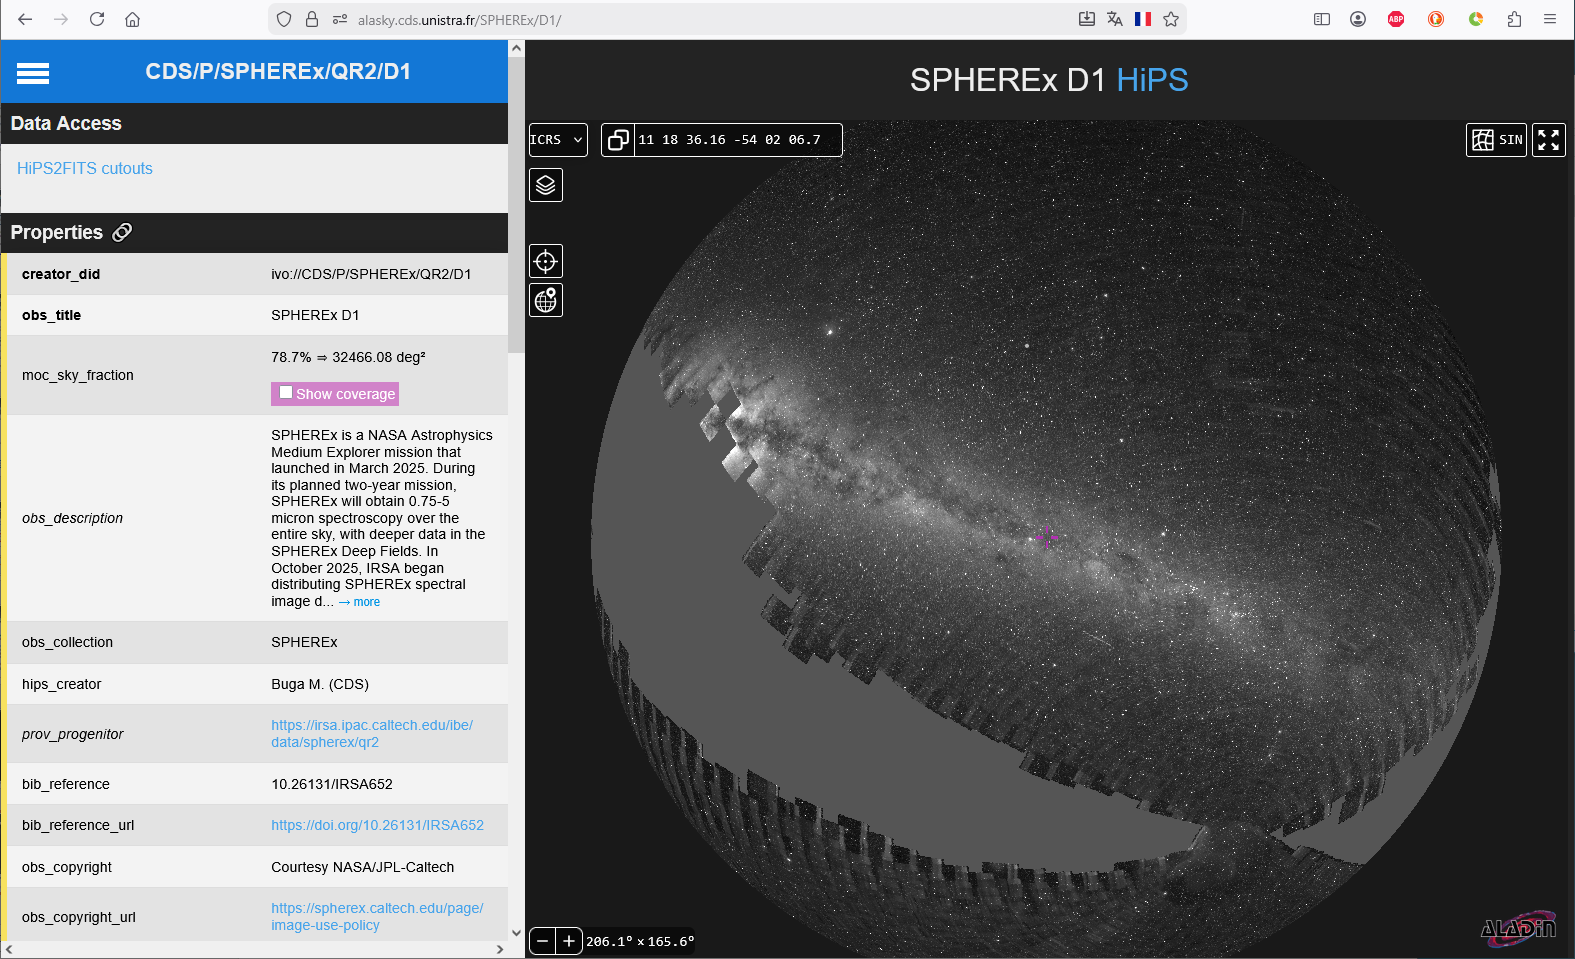
\includegraphics[width=\textwidth]{HiPS-f18.png}
\end{center}
\caption{Example of index.html file generated by Aladin/Hipsgen tool displayed in a Web browser}
\label{fig:fig18}
\end{figure}

\section{HiPS distribution and registration}
\label{sec:distribution}

This section describes the notions of HiPS node, HiPS list and HiPS registration required for the building of the HiPS distribution system.
A HiPS may be used locally by a dedicated client, in which case no distribution or registration mechanism are required. However HiPS are usually published on-line so that remote clients can access them. These clients need to know the existence and the location of the available HiPS. It is also possible to have duplicated HiPS at different locations to ensure continuity and faster access.

\subsection{HiPS node}

A HiPS node is a regular HTTP site which provides HiPS surveys. As HiPS are seen as a simple hierarchy of directories and files, the distribution of HiPS may be operated by publishing the HiPS file structures via the HTTP server. However the actual implementation of HiPS as directories and files is not an obligation, only the view as directories and files is required. Behind the HTTP server, a HiPS may be stored in a database, or any other appropriate method for packaging it (tar, zip or specific binary files…) rather than a basic file system directory.

%\underline{Note:} According to the HTTP site configuration, the tiles, notably the FITS tiles, may or may not be compressed. So it is up the clients to ensure that the required uncompression step is performed (as can be done transparently by the HTTP libraries)

Additionally, a HiPS node must implement a dedicated URL which provides the list of the HiPS surveys following the HiPS list syntax described in the next section.

\subsection{HiPS list}
\label{sec:hipslist}

A HiPS list is the list of HiPS surveys published by a given HiPS node. The HiPS list must be provided by any HiPS node via a dedicated URL.
The format of this list is derived from the HiPS properties file associated to each HiPS.  It is an UTF-8 file containing a collection of records (key1 = property1 \textbackslash n key2 = property2...) that are separated by blank lines and have the same syntax and vocabulary as the HiPS properties file. 
Each record of the HiPS list must provide at least these four mandatory properties: {\bf creator\_did, hips\_release\_date, hips\_service\_url, hips\_status}. Other HiPS properties may or may not be provided (see the list of keywords in table~\ref{tab:keywords}).

\begin{tcolorbox}[title=Example of a HiPS list]
\begin{verbatim}
# Hipslist of http://alasky.cds.unistra.fr HiPS node
creator_did          = ivo://CADC/P/HST/F850LP/r3
hips_release_date    = 2014-10-14T12:00Z
hips_service_url     = http://alasky.cds.unistra.fr/F850LP
hips_status          = public master clonable

creator_did          = ivo://CDS/P/2MASS/H
hips_release_date    = 2014-11-03T12:00Z
hips_service_url     = http://alasky.cds.unistra.fr/2MASS/H
hips_status          = public mirror unclonable
hips_estsize         = 1610612736IDs2007
hips_order           = 9
hips_tile_format     = fits jpeg
dataproduct_type     = image
moc_sky_fraction     = 1

...
\end{verbatim}
\end{tcolorbox}

\begin{tcolorbox}
\underline{Best practice: } A HiPS list may be easily generated as the concatenation of the properties files  \footnote{In this case, the possible blank lines inside a properties file must be removed.} of all distributed HiPS, with blank line separators.
\end{tcolorbox}

\subsection{HiPS registration}

HiPS surveys and/or HiPS nodes may be registered in the IVOA registry \citep{2008ivoa.spec.0222P}. 
HiPS registration in the IVOA registry may occurs at two different levels:
\begin{itemize}[noitemsep,topsep=0pt,parsep=0pt,partopsep=0pt]
   \item Individual HiPS survey registration could be useful to at least get a valid IVOID identifier \citep{2016ivoa.spec.0523D}. However this step is not required for client visibility;
   \item HiPS node registration allowing HiPS clients to discover all the HiPS via their HiPS list.
Only the HiPS node registration is required in order to be visible through compatible clients. The HiPS clients get the HiPS list for each registered HiPS node in order to compute the list of available HiPS surveys, their location, and their potential mirror sites.
\end{itemize}

\begin{tcolorbox}
\underline{Best practice: } This task may be done by an intermediate registry tool (HiPS list aggregator) which maintains an up-to-date merging of all available HiPS lists \footnote{An example of this aggregator service can be used thanks to these URLs: ASCII result: https://aladin.cds.unistra.fr/hips/globalhipslist, JSON result: https://aladin.cds.unistra.fr/hips/globalhipslist?fmt=json}. This approach is similar to the Global TAP schema aggregator described in section 3.1 of the IVOA "Discovering Data Collections" note \citep{DiscoverCollections2016}.
\end{tcolorbox}

\begin{figure}[h]
\begin{center}
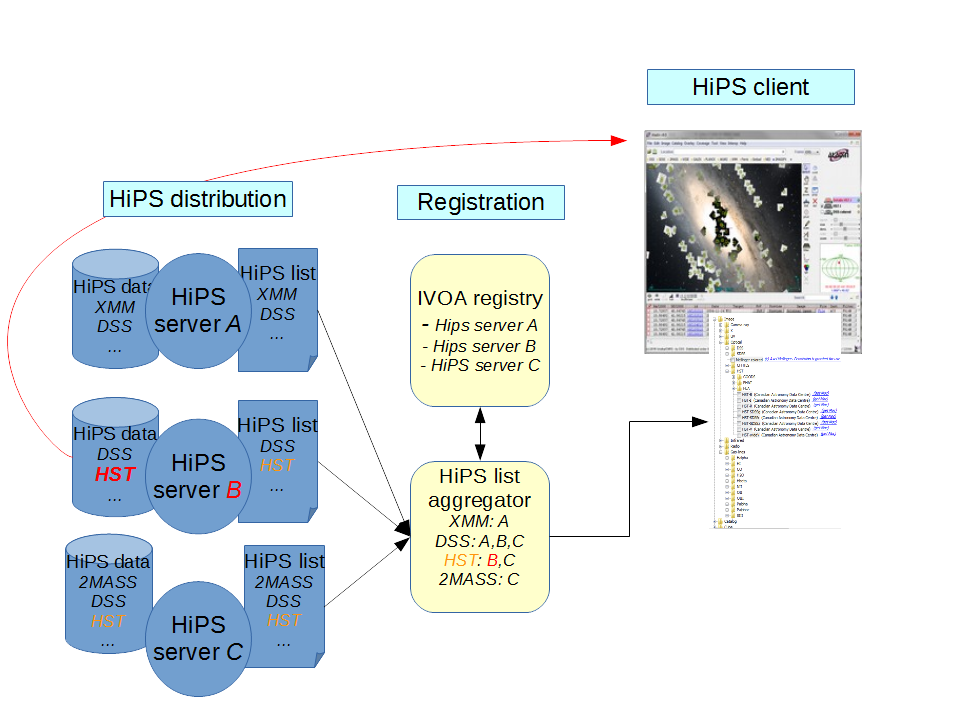
\includegraphics[width=\textwidth]{HiPS-f19.png}
\end{center}
\caption{HiPS client discovering principle}
\label{fig:fig19}
\end{figure}

\subsubsection{HiPS node registration}
A HiPS node may be registered in the IVOA registry by using an IVOA XML record declaration. This record must provide the capability of the HiPS list URL associated to the declared HiPS node by using the standardID: "{\bf ivo://ivoa.net/std/hips\#hipslist-1.0}"

{\footnotesize
\begin{verbatim}
<ri:Resource xmlns:(...) xsi:type="vr:Service">
   <title>CDS HiPS Service (master server)</title>
   <shortName>CDS hipsmaster</shortName>
   <identifier>ivo://CDS/hipsmaster</identifier>
   <curation>
       <publisher>CDS</publisher>
       <creator>
           <name>Centre de Donnees astronomiques de strasbourg</name>
        </creator>
        <contact>
           <name>CDS Helpdesk</name>
           <email>cds-question@unistra.fr</email>
       </contact>
   </curation>
   <content>
       <subject>CDS Hierarchical Progressive Surveys</subject>
       <description>The CDS provides a collection of reference
          surveys available thanks to HiPS protocol...</description>
       <referenceURL>http://aladin.cds.unistra.fr/hips</referenceURL>
       <type>Archive</type>
       <contentLevel>Research</contentLevel>
   </content>
   <capability standardID="ivo://ivoa.net/std/hips#hipslist-1.0">
      <interface role="std" xsi:type="vs:ParamHTTP">
        <accessURL use="full" >
           http://alasky.cds.unistra.fr/hipslist</accessURL>
      </interface>
   </capability>
</ri:Resource>
\end{verbatim}
}

\subsubsection{Individual HiPS survey declarations}
Optionally, each HiPS may be registered individually in the IVOA registry. There are two constraints:
\begin{itemize}[noitemsep,topsep=0pt,parsep=0pt,partopsep=0pt]
\item Only the main HIPS creator is authorized to register them (and not by the potential clone site manager),
\item Only the URL of the original HiPS (master site, not the clone site) may be provided by using the standardID: "{\bf ivo://ivoa.net/std/hips\#hips-2.0}" \footnote{or "{\bf ivo://ivoa.net/std/hips\#hips-1.0}" for a reference to the previous HiPS document recommendation.}
\end{itemize}

{\footnotesize
\begin{verbatim}


<ri:Resource xmlns:(...) xsi:type="vs:CatalogService">
   <title>ALADIN image DSS2 blue survey collection</title>
   <shortName>Aladin DSS2 blue</shortName>
   <identifier>ivo://CDS/P/DSS2/blue</identifier>
   <curation>
     <publisher>CDS</publisher>
     <creator ivo-id="ivo://CDS">
       <name>Centre de Donnees astronomiques de strasbourg</name>
     </creator>
     <contact>
        <name>CDS Helpdesk</name>
        <email>cds-question@unistra.fr</email>
     </contact>
   </curation>
   <content>
     <subject>ALADIN image DSS2 blue survey collection</subject>
     <description> ALADIN image server provides reference ... </description>
     <referenceURL>http://aladin.cds.unistra.fr</referenceURL>
     <type>Survey</type>
     <contentLevel>Research</contentLevel>
   </content>
   <capability standardID="ivo://ivoa.net/std/hips#hips-2.0">
     <interface role="std" xsi:type="vs:ParamHTTP">
       <accessURL use="base">
          http://alasky.cds.unistra.fr/DSS/DSS2-blue-XJ-S</accessURL>
     </interface>
   </capability>
   <coverage>
      <footprint ivo-id="ivo://mocivod">
         http://alaskycds.unistra.fr/DSS/DSS2-blue-XJ-S/Moc.fits
      </footprint>
   </coverage>
 </ri:Resource>
\end{verbatim}
}

\subsection{HiPS mirroring}

HiPS surveys are governed by usual data rights policies. The data may be public or private. It may be mirrored or not, according to the original data rights rules set by the HiPS creator (see hips\_licence propertie keyword)  .
If both the original data copyright statement and the HiPS creator authorize the duplication and the distribution of any derived HiPS products, it could be interesting to mirror HiPS in order to provide faster and more secure access.
Any HiPS node – having full copy and distribution rights - may mirror a HiPS survey from other HiPS node on condition that the HiPS survey is described by the HiPS node list, and with the explicit property "hips\_status = … clonable … ".
A HiPS node which provides a copy of a HiPS survey must specify "hips\_status = … mirror ..." for the clone. If the "hips\_status" was originally "… clonableOnce …" it must replace it by "… unclonable …" to avoid a new copy from this mirror. If the mirroring is partial (lower hips\_order, or only a subset of tile formats), the server who has done the mirroring must specify "hips\_status = … partial …", and adjust the relevant properties accordingly (hips\_service\_url, hips\_order, hips\_tile\_format), in its HiPS list and in the "properties" file of the concerned HiPS.
A HiPS node which provides a copy of a HiPS survey must not modify the hips\_release\_date of the master site in order to detect out of date copies.

There is no dedicated protocol for the HiPS mirroring process. It can be done via wget, rsync, Hipsgen or any other method used for synchronized HTTP web sites. 


\section{HiPS access and use}
\label{sec:use}

This section is not normative. It describes the procedures that a HiPS client may implement to access and use HiPS.
HiPS allows a wide range of usages. One could use the HIPS surveys in a dedicated window as part of a web application or one could use the HIPS client to find areas of interest using the tiles and then retrieve them in FITS format to gain access to their full dynamic range. With its open and simple architecture, usage is left to the imagination of the users and the capabilities of the client.

\subsection{Local access}

Some HiPS clients are capable of displaying a locally stored HiPS by using its root directory file name and deriving the file names of the various HiPS components (tiles, properties, MOC etc.). In this mode, there is no need to provide registry access or cache management. Only the knowledge of the HiPS root directory is required. Tiles and properties, and additional metadata file paths are directly derived and defined from the HiPS root directory path. Usually, the properties file is read first by the client in order to know the required HiPS parameters and limits (HiPS deepest order, tile formats, coordinate system reference, etc).

\begin{itemize}
\item properties file $\rightarrow$ rootDir/properties
\item Tiles $\rightarrow$ {\em rootDir}/NorderK/DirD/NpixN\{.ext\}
where K is the order, N tile index, D=(N//10000)*10000,
\{.ext\} is .fits, .jpg, .png, …
\item MOC file $\rightarrow$ {\em rootDir}/Moc.fits
\item Allsky files $\rightarrow$ {\em rootDir}/NorderK/Allsky\{.ext\}
where K is the order, {.ext} is .fits, .jpg, .png, …
\item etc.
\end{itemize}

Example: the FITS tile containing the HiPS data corresponding to the HEALPix cell index 10302 at the order 6 will be available through this relative path ./Norder6/Dir10000/Npix10302.fits


\subsection{Remote access}

Most of the HiPS clients use remote access through the Internet. In this mode, the HiPS structure is read using the HTTP protocol.  Since the remote client knows the base URL of a dedicated HiPS, it can directly query the properties, tiles and the various additional elements of the HiPS structure.

\begin{itemize}
\item properties file $\rightarrow$ {\em baseURL}/properties
\item Tiles $\rightarrow$ {\em baseURL}/NorderK/DirD/NpixN\{.ex\}
where K  is the order, N tile index, D=(N//10000)*10000,
\{.ext\} is .fits, .jpg, .png, …
\item MOC file $\rightarrow$ {\em baseURL}/Moc.fits
\item Allsky files $\rightarrow$ {\em baseURL}/NorderK/Allsky\{.ext\}
where K is the order, \{.ext\} is .fits, .jpg, .png, …
\item etc.
\end{itemize}

Example: the FITS tile containing the HiPS data corresponding to the HEALPix cell index 10302 at the order 6 located on "path/of/myhips" HTTP location on "myhostname" server will be available through this URL \\ http://myhostname/path/of/myhips/Norder6/Dir10000/Npix10302.fits

The client knowledge of any available HiPS, their name, their base URL and possibly their mirror sites, may be read through the IVOA registry declarations (see section~\ref{sec:distribution}). 

In the case of remote HiPS access, it is strongly recommended that the client implement a cache mechanism to minimize load on the HiPS nodes.

There is no recommended HiPS authentification and/or encryption mechanism. As remote HiPS access is based on any regular HTTP server, any usual HTTP/HTTPS authentification and encryption method may be applied if required \citep{SSO2008}.

\subsection{Suggested display algorithms}

There is no recommended HiPS client display algorithm. The best HiPS display algorithms depends on the goal of the client.

The main goal of the display algorithm is to draw the relevant tiles at the appropriate resolution for a particular sky region. The larger the sky region, the more complex the display algorithm will need to be in order to take into account the distortions due to the spherical projection whatever this projection is (sinus, tangential, aitoff, mollweide, etc…).

The three next sections will discuss three display algorithms for HIPS images, HiPS catalogues and HiPS cubes which could be adapted according to different scientific goals.

\subsubsection{Algorithm for drawing HiPS image}

The best HiPS display strategy is usually a balance between the drawing speed and the display quality. The following is an example of the basic algorithm, with emphasis on a number of improvements.

\subparagraph{Basis of the algorithm}
For a given sky region (typically a rectangle area corresponding to the client display window):
\begin{enumerate}
\item Compute the relevant HiPS order (one screen pixel should be cover by one tile pixel)
\item Compute the list of HEALPix tile indices covering the region (HEALPix lib function)
\item Retrieve the corresponding tiles (locally or via the Internet)
\item Draw each tile on the corresponding sky location based of the associated HEALPix cell. The fast method uses only the 4 corners of the HEALPix cell and draw the tile in two complementary triangles (clipping required) mapping the bilinear stretch of the tile. This drawing step may be improved in quality by using more control points than the 4 corners by subdividing each tile in sub HEALPix cells and by this way, reduce the projection distortions.
\end{enumerate}

\subparagraph{Allsky usage improvement}
The client drawing a HiPS at low resolutions (order 0 to 3) should first determine whether a Allsky.xxx file exists in the NorderK directory, and if yes, it should load it, split it as a collection of very low resolution tiles, and draw them. A client could also decide to use the regular individual NorderK tiles as an intermediate zoom level before drawing the Norder(K+1) tiles.

\subparagraph{Moc.fits usage improvement}
A client may use the Moc.fits file to avoid loading any HiPS tiles located outside the HiPS coverage (intermediate step between 2 and 3 in the previous algorithm).

\begin{figure}[h]
\begin{center}
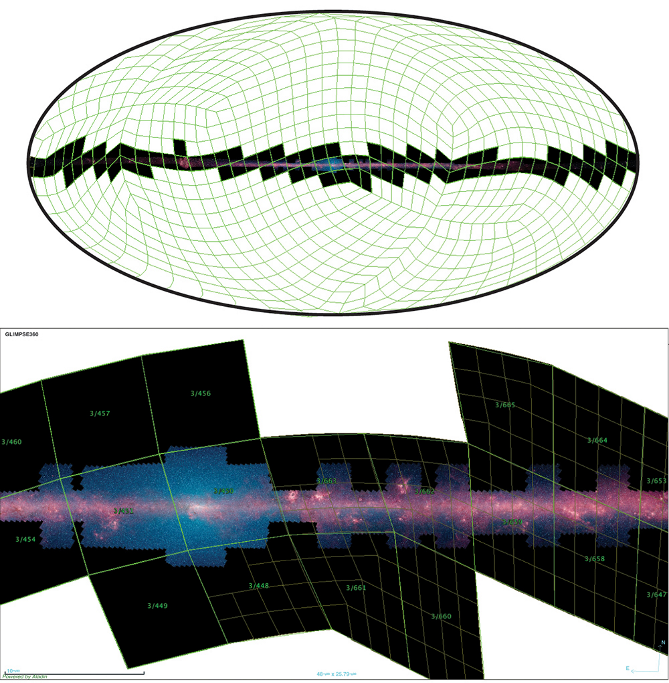
\includegraphics[width=\textwidth]{HiPS-f20.png}
\end{center}
\caption{HiPS tiles of Glimpse colored survey}
\label{fig:fig20}
\end{figure}

\subsubsection{Algorithm for drawing HiPS catalog}

The algorithm for drawing HiPS catalog is simpler to implement than the one for the HiPS image because the catalogue tiles are just used as a container where the sky position for of each source in the catalogue is provided explicitly.
 
\subparagraph{Basis of the algorithm}
For a given sky region, from the lower order:
\begin{enumerate}
\item Compute the list of HEALPix tile indices covering the region (HEALPix lib function)
\item Retrieve the corresponding tiles (locally or via the Internet)
\item Draw the sources inside the tiles (position on the sky and/or associated measurement information)
\item Continue with the next order if required (depending of the algorithm: number of drawn sources, order number compared to the view size…)
\end{enumerate}


\subparagraph{Allsky usage improvement}
The client which displays a HiPS catalog at low resolution (order 0 to 3) may look first if a Allsky.xxx is existing in the NorderK, and if yes, it should load it and display the corresponding sources. In this case, the regular NorderK tiles must be ignored for avoiding duplicates sources. 

\subparagraph{Moc.fits usage improvement}
A client may use the Moc.fits file to avoid loading the HiPS tiles outside the HiPS coverage (intermediate step between 2 and 3 in the previous algorithm).

\subparagraph{metadata.xml usage improvement}
A client may use the metadata.xml file for knowing the descriptions, the units and other related metadata associated to the HiPS catalog.

\subsubsection{Algorithm for drawing HiPS cube}

For the readibility of this section, the description of the algorithm for visualizing a HiPS cube will assume a spatial-frequency case. The same algorithm can be used for any other type of HiPS cube.

The choice of algorithm for visualizing a HiPS cube depends on how the client performs such visualization. Below, we describe the simplest method, which consists of simultaneously visualizing the two physical components: the spatial component corresponding to a specific frequency of the cubic data, and the frequency component in the form of a portion of spectrum associated with the position of the central pixel of the spatial view. It is up to the visualization client to adjust the spatial view in case of zooming or changing the cubic channel, and conversely to modify the spectrum view in case of zooming or panning the spatial view.

\begin{figure}[h]
\begin{center}
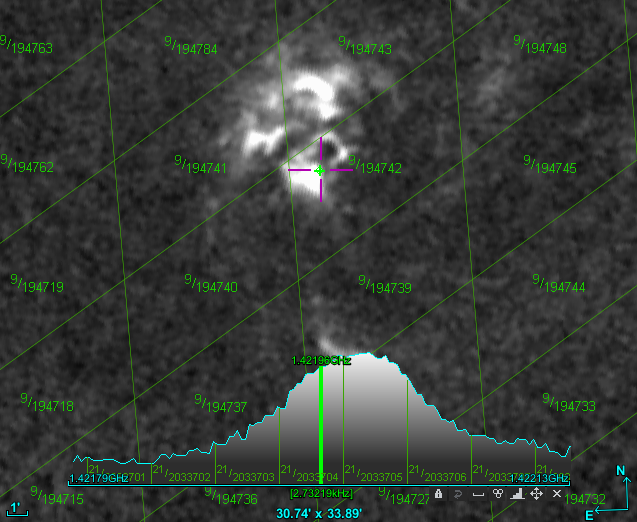
\includegraphics[width=\textwidth]{HiPS-f22.png}
\end{center}
\caption{Basic HiPS cube visualisation algorithm}
\label{fig:fig22}
\end{figure}

\subparagraph{Basis of the algorithm for the spatial component}

The visualization of the spatial component follows the same principle as for a standard HiPS image: the angular size of the field of view to be displayed determines the spatial order and the indices of the HiPS tiles to be drawn.  This will be done for a given frequency determined by the visualization client. That frequency is converted into an index according to the discretization function recommended in this document. The most basic algorithm determines the frequency order directly from the spatial order using the formula orderF = orderMaxF - (orderMaxS - OrderS) by considering orderMaxS and orderMaxF as the deepest orders for both components, orderS and orderF as the current orders. Then, for each tile covering the spatial field of view, it is easy to extract the channel corresponding to the frequency index and, from there, visualize the field of view.

\subparagraph{Basis of the algorithm for the frequency component}

The visualization of the spectral component follows the same logic as for spatial visualization: it involves plotting a "portion" of the spectrum by choosing a frequency order adapted to the number of channels that can be displayed in this frequency interval. The spectrum is typically displayed on a straight line segment representing the frequency axis. Considering that the frequency order is linked—in a first approximation—to the spatial order, the limits of the frequency interval will be derived from the chosen order. Thus for a given frequency range and for a dedicated target spatiale position:
\begin{enumerate}
\item Calculate the spatial index covering the target position;
\item Determine the minimum and maximum frequencies that can be displayed at the corresponding resolution.
\item Calculate the list of corresponding frequency indices
\item Retrieve the tiles corresponding to these indices for the target position
\item Plot the spectrum values on the frequency axis extracted from the tiles at the target position.
\end{enumerate}

\subparagraph{Moc.fits usage improvement}

A client may use the Moc.fits file to avoid loading any HiPS tiles located outside the HiPS coverage (in space and in frequency).

\subparagraph{A few basic improvements}

Basic improvements can be applied to the algorithm above. The first consists of tracing the spectrum not for a single target spatial pixel, but for all pixels within a certain angular radius. This method allow to obtain an integrated spectrum. The plotting time is similar because most of the adjacent pixels come from the same HiPS tiles. 

A second improvement consists of decoupling the frequency order from the spatial order. By this way, it is possible to zoom independently on the spatial view or the frequency view in order to visualize, for example, the entire spectrum while showing a small spatial coverage. Or, conversely, to display a high-resolution spectrum over a very large spatial field of view. This improvement depends on the combinations of HiPS tiles available on the HiPS node. If the corresponding orders are not available, it is up to the client to display an oversampled or undersampled spectrum (or spatial view, respectively). 

If the keyword obs\_restfreq is specified in the "properties" file, the client can choose to display in speed unit rather than frequencies or wavelengths.


\section{Conclusion and perspectives}

In conclusion, the IVOA HiPS standard provides a powerful and flexible framework for the efficient organization, storage, and access of astronomical data through multi-resolution discretization.  This approach enhances query performance and data exploration while preserving information richness.
The document focuses specifically on spherical or spherico-cubic data. However, the HiPS method could be relatively easily adapted to non-spherical data—such as purely temporal or frequency-based datasets—where hierarchical access would be justified (e.g., for very large time series or spectra).
While primarily designed for celestial observations, HiPS is also applicable to planetary surface data or any dataset described in spherical or cubico-spherical coordinates. Beyond its emphasis on visualization, HiPS serves as a generalized framework for mapping data into a unified architecture, thereby enabling a wide range of scientific use cases, particularly those involving the comparison and combination of surveys.



% NOTE: IVOA recommendations must be cited from docrepo rather than ivoabib
% (REC entries there are for legacy documents only)
\bibliography{HiPS.bib,ivoatex/ivoabib,ivoatex/docrepo}

\appendix

\section{Basic rules and formulae useful for HiPS manipulations.}

\subsection{Spatial case}

\begin{itemize}
\item Hierarchy path of tile \\
Tile N in order K $\rightarrow$ NorderK/DirD/NpixN\{.ext\}
  where $ D=(N//10000) \times 10000 $,\\
  and \{.ext\} is depending of the file format of the tiles (.fits, .jpg, .png …)
\item Parent of the tile\\
Tile N in order K $\rightarrow$ Direct parent order K-1: tile N//4
\item 4 children of the tile\\
Tile N in order K $\rightarrow$ Children order K+1: tiles Nx4, Nx4+1, Nx4+2, Nx4+3
\item Number of HEALPix cells on the whole sphere\\
Order K $\rightarrow$ $ 12 \times 2^K \times 2^K $
\item HEALPix cell angular size (global average)\\
HEAlPix cell radian angular size at order K =~ $ \sqrt( 4 \times PI / (12 \times 2^K \times 2^K) $
\item Spherical coordinate of a HEALPix cell (center)\\
Cell indice N, order K $\rightarrow$ (lon,lat): requires a HEALPix method :\\
(lon,lat) = HEALPix\_pix2ang\_nested(N,K)
\item Spherical coordinates of a HEALPix cell (4 corners)\\
Cell indice N, order K $\rightarrow$ (lon0,lat0,…lon3,lat3): requires a HEALPix method:\\
(lon0,lat0,…lon3,lat3) = HEALPix\_pix2corners\_nested(N,K)
\item HEALPix cell containing a spherical coordinate\\
(lon,lat), order K $\rightarrow$ Cell indice N: requires a HEALPix method:\\
N = HEALPix\_ang2pix\_nested(lon,lat,K)
\item HiPS image size vs original image collection size\\
HiPS size $\rightarrow$ ~ 1.3x the original image collection \\
(without overlay and without hole in original image collection, using the same coding (BITPIX) and the same pixel angular resolution).
\item HiPS image size order K vs HiPS size order K+1\\
HiPS size order K $\rightarrow$ ~ 0.25x HiPS size order K+1
\item HiPS catalog size vs original catalog size\\
HiPS size ~= original catalog size
\end{itemize}

\subsection{Cubic case}
\label{sec:cubicFormula}

\begin{itemize}
\item Hierarchy path of tile (frequency case, same for temporal)\\
Tile N in order K (space), M in order L (frequency), \\
$\rightarrow$ NorderK\_L/DirD\_E/NpixN\_M\{.ext\}\\
  where $ D=(N//10000) \times 10000, E=(M//10) \times 10 $,\\
  and \{.ext\} is depending of the file format of the tiles (.fits, .jpg, .png …)
\item HiPS cube size vs original cube collection size\\
HiPS size $\rightarrow$ ~ 1.15x the original cube collection \\
(without overlay and without hole in original cube collection, using the same coding (BITPIX) and the same pixel resolution).
\item HiPS cube size order K vs HiPS size order K+1 (default resolutions)\\
HiPS size order K $\rightarrow$ ~ 0.125x HiPS size order K+1
\item Time dimension discretization\\
Time index at order 61 $\rightarrow$ JD expressed in microseconds
\item Frequency dimension discretization\\
Freq index at order 51  $\rightarrow$  $  \left\lfloor ( \log_{10}(\textit{freq}) + 18 )/ {56} ) \times 2^{52}   \right\rfloor $
\item Parent of the tile (frequency case, same for temporal)\\
Tile N in order K (space), M in order L (frequency),\\
$\rightarrow$ Space direct parent order K-1: tile N/4\\
$\rightarrow$ Frequency direct parent order L-1: tile M//2
\item 8 children of the tile (frequency case, same for temporal)\\
Tile N in order K (space), M in order L (frequency),\\
$\rightarrow$ Space children order $K+1: tiles N \times 4, N \times 4+1, N \times 4+2, N \times 4+3$\\
$\rightarrow$ Frequency children order $L+1: tiles M \times 2, M \times 2+1$

%\item Suggested time WCS keywords values for the tile of indice M in order L, for a depth = $2^{orderInTile}$:\\
%   CTYPE3 = 'TIME'\\
%   TIMESYS = 'TDB'\\
%   JDREF = $ ( M * 2^{orderInTile} ) / 86400 $\\
%   CUNIT3 = 's'\\
%   CRPIX3 = 1\\
%   CRVAL3 = 0\\
%   CDELT3 = 1.0E-6 * 2^{61 - L}

\item Suggested time WCS keywords values for the tile of indice M in order L, for a depth equals to $2^{orderInTile}$:\\
{\ttfamily
CTYPE3   = 'TIME'\\
TIMESYS = 'TDB'\\
JDREFI    = $(M \times 2^{orderInTile}) // 86400$\\
JDREFF   = $((M \times 2^{orderInTile}) \% 86400) / 86400$\\
CUNIT3   = 's'\\
CRPIX3   = 1\\
CRVAL3  = 0\\
CD3\_3    = $1.0E-6 \times 2^{61 - L}$
}
\item Suggested frequency WCS keywords values for the tile of indice M in order L, for a depth equals to $2^{orderInTile}$:\\
{\ttfamily
CTYPE3  = 'FREQ-LOG'\\
CUNIT3  =' Hz'\\
CRPIX3  = $1 - ( M \times 2^{orderInTile}$ )\\
CRVAL3 = $1E-18$\\
CD3\_3   = $1E-18 \times ( log(1E+38/1E-18) / 2^{(L+orderInTile)} )$
}
\end{itemize}


\section{Generic HiPS cube extension}
\label{sec:generic}

This document provides a normative description of HiPS cubes for spatio-temporal or spatio-frequency data. This appendix proposes a possible, but non-standardized, extension to describe any collection of cubes if it is not possible to convert the additional dimension into Hertz or TDB reference microseconds. It should be noted, however, that such use will, by design, limit the usage, as it will not be easily comparable or combinable with another HiPS.

The suggested method is to use the "properties" file to describe the parameters characterizing the discretization function used in the generic HiPS cube. We propose the keywords associated with the following formulas:

\paragraph{Linear discretisation:}

The original values must be expressed as integers between 0 and $2^{61}-1$ included.

\begin{tcolorbox}
\begin{verbatim}
data_product_type = generic-cube
hips_ctype3       = axisType (string)
hips_ref          = origin (number)
hips_cunit3       = unit (string)
\end{verbatim}
\end{tcolorbox}

The discretization for a given value, expressed in the specified unit, for a given order is calculated using the following formula:

\medskip
\noindent\fbox{%
\parbox{0.98\linewidth}{%
\centering
\[
index = \lfloor (value - origin) / 2^{61-order} \rfloor 
\]
}}
\medskip

\paragraph{Logarithmic discretisation}

The original values must be expressed between 1.0E-18 and 1.0+38.

\begin{tcolorbox}
\begin{verbatim}
data_product_type = generic-cube
hips_ctype3       = axisType-log (string)
hips_cunit3       = unit (string)
 \end{verbatim}
\end{tcolorbox}

The discretization for a given value, expressed in the specified unit, for a given order is calculated using the following formula:

\medskip
\noindent\fbox{%
\parbox{0.98\linewidth}{%
\centering
\[
\mathrm{index}
= \left\lfloor 2^{order} \cdot \frac{\log_{10}(\mathrm{value}) + 18}{56} \right\rfloor 
\]
}}
\medskip


\section{Version History}
\label{sec:history}

% \subsection{Changes between versions 1.0 and 2.0}

The differences between version 2.0 of HiPS and the preceding version 1.0 are fully dedicated to the extension/generalisation of the HiPS hierarchy principle to cubic data. 

It should be noted that the previous version 1.0 described a more basic method for generating HiPS cubes in specific cases where the original cubes were perfectly homogeneous in terms of the physical meaning of the channels. This method has been replaced by the new recommendations related to HiPS cubes. However, although this previous method is now deprecated, it can still be used as it is compatible with the cubic extensions described in this document.

This major version also included minor changes and clarifications to the previous text:
\begin{itemize}[noitemsep,topsep=0pt,parsep=0pt,partopsep=0pt]
   \item A glossary of vocabulary specific to HiPS has been added before the standardized sections;
   \item Two possible "enablers" for FITS tiles have been introduced: the removal of unused edges (TRIM), and the addition of WCS keywords;
   \item The choice of the equatorial reference frame as the default for spatial HiPS has been reinforced;
   \item The choice of the MOC reference system has been clarified, according to the new MOC document \citep{MOC2.1};
%   \item The formula for calculating angular size form order is now expressed in degrees rather than radians, and the reciprocal formula is indicated;
   \item  Alternatives for tile encoding, notably WEBP and RICE FITS, have been mentioned, along with the associated constraints;
   \item The table of suggested keywords has been cleaned, notably some very specific suggested clients key words have been removed of this document, rearranged, and some new key words have been introduced.
\end{itemize}


\end{document}
